\documentclass{article}


% if you need to pass options to natbib, use, e.g.:
%     \PassOptionsToPackage{numbers, compress}{natbib}
% before loading neurips_2023


% ready for submission
% \usepackage[nonatbib]{neurips_2023}


% to compile a preprint version, e.g., for submission to arXiv, add add the
% [preprint] option:
%     \usepackage[preprint]{neurips_2023}


% to compile a camera-ready version, add the [final] option, e.g.:
\usepackage[final,nonatbib]{neurips_2023}


% to avoid loading the natbib package, add option nonatbib:
%    \usepackage[nonatbib]{neurips_2023}


% Include other packages here, before hyperref.
\usepackage{microtype}      % microtypography
\usepackage{graphicx}
\usepackage{tikz}
\usepackage{xfp}
%\usepackage[utf8]{inputenc} % allow utf-8 input
%\usepackage[T1]{fontenc}    % use 8-bit T1 fonts
%\usepackage{hyperref}       % hyperlinks
\usepackage{url}            % simple URL typesetting
\usepackage{booktabs}       % professional-quality tables
\usepackage{amsfonts}       % blackboard math symbols
\usepackage{nicefrac}       % compact symbols for 1/2, etc.
\usepackage{xcolor}         % colors
\usepackage{amsmath}
\usepackage{amssymb} 
\usepackage{amsthm}         % proof environment
% \usepackage{algorithm}
% \usepackage{algpseudocode}
\usepackage{multirow}
\usepackage{array}          % allows "m" in tabular    
\usepackage[pagebackref,hidelinks]{hyperref}
%\hypersetup{
%    colorlinks=true,
%    linkcolor=blue,
%    filecolor=blue,      
%    urlcolor=blue,
%    citecolor=blue,
%    }

%%%%%%%%%%%%%%%%%%%%%%%%%%%%%%%%
% THEOREMS
%%%%%%%%%%%%%%%%%%%%%%%%%%%%%%%%
\theoremstyle{plain}
\newtheorem{theorem}{Theorem}[section]
\newtheorem{proposition}[theorem]{Proposition}
\newtheorem{lemma}[theorem]{Lemma}
\newtheorem{corollary}[theorem]{Corollary}
\newtheorem{conjecture}{Conjecture}
\theoremstyle{definition}
\newtheorem{definition}[theorem]{Definition}
\newtheorem{assumption}[theorem]{Assumption}
\theoremstyle{remark}
\newtheorem{remark}[theorem]{Remark}

%------------------------------------------------------------------
 % math shortcuts
 \renewcommand{\tilde}{\widetilde}
 \renewcommand{\hat}{\widehat}
 \renewcommand{\bar}{\overline}
 %\newcommand{\defn}{\ensuremath{:=}}
 \newcommand{\defn}{\triangleq}
 \newcommand{\limit}[2]{\ensuremath{\lim_{#1 \rightarrow #2}}}
 \newcommand{\bvec}[1]{\ensuremath{\Breve{\boldsymbol{#1}}}}
 \newcommand{\tvec}[1]{\ensuremath{\Tilde{\boldsymbol{#1}}}}
 \newcommand{\uvec}[1]{\ensuremath{\underline{\boldsymbol{#1}}}}
 \newcommand{\ovec}[1]{\boldsymbol{\Bar{#1}}}
 \newcommand{\hvec}[1]{\ensuremath{\Hat{\boldsymbol{#1}}}}
 \renewcommand{\vec}[1]{\ensuremath{\boldsymbol{#1}}}
 \newcommand{\huvec}[1]{\ensuremath{\Hat{\underline{\boldsymbol{#1}}}}}
 \newcommand{\hovec}[1]{\ensuremath{\Hat{\Bar{\boldsymbol{#1}}}}}
 \newcommand{\mat}[1]{\ensuremath{\begin{bmatrix}#1\end{bmatrix}}}
 \newcommand{\smallmat}[1]{\ensuremath{
        \left[\begin{smallmatrix}#1\end{smallmatrix}\right]}}
 \newcommand{\ip}[1]{\ensuremath{\left\langle #1 \right\rangle}}
 %\newcommand{\ip}[1]{\mbox{$<$}#1\mbox{$>$}}
 \newcommand{\norm}[1]{\ensuremath{\| #1 \|}}
 \newcommand{\mc}[1]{\ensuremath{\mathcal{#1}}}
 \newcommand{\st}{{~\text{s.t.}~}}
 \newcommand{\barst}[1]{\ensuremath{\text{\raisebox{-0.5mm}{$\bigl|_{#1}$}}}}
 \newcommand{\Barst}[1]{\ensuremath{\text{\raisebox{-0.5mm}{$\biggl|_{#1}$}}}}
 \newcommand{\zci}{{\textstyle\frac{1}{z^*}}}
 \newcommand{\Real}{{\mathbb{R}}}
 \newcommand{\Complex}{{\mathbb{C}}}
 \newcommand{\Int}{{\mathbb{Z}}}
 \newcommand{\Nat}{{\mathbb{N}}}
 \newcommand{\Rat}{{\mathbb{Q}}}
 \newcommand{\Field}{\mathbb{F}}
 \newcommand{\Ell}{\mathcal{L}}
 \newcommand{\Expectation}{\mathbb{E}}
 \newcommand{\conv}{\ast}
 \newcommand{\cconv}{\circledast}
 \newcommand{\of}[1]{^{\scriptscriptstyle (#1)}}
 \newcommand{\oft}[1]{^{{\scriptscriptstyle (#1)}t}}
 \newcommand{\ofc}[1]{^{{\scriptscriptstyle (#1)}*}}
 \newcommand{\ofH}[1]{^{{\scriptscriptstyle (#1)}H}}
 \newcommand{\modulo}[1]{\left\langle #1 \right\rangle}
 \newcommand{\floor}[1]{\left\lfloor #1 \right\rfloor}
 \newcommand{\ceil}[1]{\left\lceil #1 \right\rceil}
 \newcommand{\iddots}{\reflectbox{$\ddots$}}
 \newcommand{\tran}{^{\top}}
 \newcommand{\herm}{^{\textsf{H}}}
 \newcommand*\deriv{\mathop{}\!\mathrm{d}}

 % operators
 \DeclareMathOperator{\real}{Re}
 \DeclareMathOperator{\imag}{Im}
 \DeclareMathOperator{\sgn}{sgn}
 \DeclareMathOperator{\csgn}{csgn}
 \DeclareMathOperator{\E}{E}
 \DeclareMathOperator{\Cov}{Cov}
 \DeclareMathOperator{\var}{var}
 \DeclareMathOperator{\kurt}{kurt}
 \DeclareMathOperator{\Kurt}{{\mc K}}
 \DeclareMathOperator{\row}{row}
 \DeclareMathOperator{\col}{col}
 \DeclareMathOperator{\spn}{span}
 \DeclareMathOperator{\tr}{tr}
 \DeclareMathOperator{\diag}{diag}
 \DeclareMathOperator{\cir}{\mc C}
 \DeclareMathOperator{\Diag}{{\mc D}}
 \DeclareMathOperator{\sinc}{sinc}
 \DeclareMathOperator{\vect}{vec}
 \DeclareMathOperator*{\argmin}{arg\,min}
 \DeclareMathOperator{\erf}{erf}

 % references
 \renewcommand{\eqref}[1]{(\ref{eq:#1})}
 \newcommand{\Eqref}[1]{Equation (\ref{eq:#1})}
 \newcommand{\Figref}[1]{Figure~\ref{fig:#1}}
 \newcommand{\figref}[1]{Fig.~\ref{fig:#1}}
 \newcommand{\tabref}[1]{Table~\ref{tab:#1}}
 \newcommand{\secref}[1]{Section~\ref{sec:#1}}
 \newcommand{\appref}[1]{Appendix~\ref{app:#1}}
 \newcommand{\lemref}[1]{Lemma~\ref{lem:#1}}
 \newcommand{\thmref}[1]{Theorem~\ref{thm:#1}}
 \newcommand{\corref}[1]{Corollary~\ref{cor:#1}}
 \newcommand{\conref}[1]{Conjecture~\ref{con:#1}}
 \newcommand{\propref}[1]{Proposition~\ref{prop:#1}}

 % colors
 \newcommand{\textr}[1]{\textcolor{red}{#1}}
 \newcommand{\textb}[1]{\textcolor{blue}{#1}}

 % statistical quantities
 \DeclareMathOperator{\SINR}{SINR}
 \DeclareMathOperator{\SIR}{SIR}
 \DeclareMathOperator{\MSE}{MSE}
 \newcommand{\mmse}{_{\mathsf{mmse}}}
 \newcommand{\pa}{p_{\mathsf{a}}}
 \newcommand{\pb}{p_{\mathsf{b}}}
 \newcommand{\pab}{p_{\mathsf{a,b}}}
 \newcommand{\px}{p_{\mathsf{x}}}
 \newcommand{\py}{p_{\mathsf{y}}}
 \newcommand{\pxy}{p_{\mathsf{x,y}}}
 \newcommand{\pygx}{p_{\mathsf{y}|\mathsf{x}}}
 \newcommand{\pxgy}{p_{\mathsf{x}|\mathsf{y}}}
 \newcommand{\pz}{p_{\mathsf{z}}}
 \newcommand{\pxh}{p_{\hat{\mathsf{x}}_{\vec{\theta}}}}
 \newcommand{\pxhgy}{p_{\hat{\mathsf{x}}|\mathsf{y}}}
 \newcommand{\Eab}{\E_{\mathsf{a,b}}}
 \newcommand{\Ey}{\E_{\mathsf{y}}}
 \newcommand{\Exgy}{\E_{\mathsf{x}|\mathsf{y}}}
 \newcommand{\Exy}{\E_{\mathsf{x,y}}}
 \newcommand{\Exhgy}{\E_{\hat{\mathsf{x}}|\mathsf{y}}}
 \newcommand{\Egy}{\E_{\hat{\mathsf{x}},y}}
 \newcommand{\Ez}{\E_{\mathsf{z}}}
 \newcommand{\Ezy}{\E_{\mathsf{z,y}}}
 \newcommand{\Exzy}{\E_{\mathsf{x,z,y}}}
 \newcommand{\Exzzy}{\E_{\mathsf{x,z_1,z_2,y}}} 
 \newcommand{\ExzPy}{\E_{\mathsf{x,z_1,...,z_P,y}}}
 \newcommand{\ExxPy}{\E_{\mathsf{x,\hat{x}_{(P)},y}}}
 \newcommand{\Eziy}{\E_{\mathsf{z_i,y}}}
 \newcommand{\Ezigy}{\E_{\mathsf{z_i}|\mathsf{y}}}
 \newcommand{\EzPgy}{\E_{\mathsf{z_1,...,z_P}|\mathsf{y}}}
 \newcommand{\EzPy}{\E_{\mathsf{z_1,...,z_P,y}}}
 \newcommand{\ExzPgy}{\E_{\mathsf{x,z_1,...,z_P}|\mathsf{y}}}
 \newcommand{\ExxP}{\E_{X,\hat{X}_1,...\hat{X}_P}}
 \newcommand{\ExP}{\E_{\hat{X}_1,...\hat{X}_P}}
 \newcommand{\Covzigy}{\Cov_{\mathsf{z_i}|\mathsf{y}}}
 \newcommand{\Covxgy}{\Cov_{\mathsf{x}|\mathsf{y}}}
 
 % GAN stuff
 \newcommand{\raw}{^{\mathsf{raw}}}
 \newcommand{\batch}{_{\mathsf{batch}}}
 \newcommand{\critic}{_{\mathsf{critic}}}
 \newcommand{\train}{_{\mathsf{train}}}
 \newcommand{\test}{_{\mathsf{test}}}
 \newcommand{\val}{_{\mathsf{val}}}
 \DeclareMathOperator{\CWD}{CWD}
 \newcommand{\Dadler}{D^{\mathsf{adler}}}
 \newcommand{\Ladler}{\mc{L}^{\mathsf{adler}}_{\mathsf{adv}}}
 \newcommand{\Ladv}{\mc{L}_{\mathsf{adv}}}
 \newcommand{\Lgp}{\mc{L}_{\mathsf{gp}}}
 \newcommand{\Ldrift}{\mc{L}_{\mathsf{drift}}}
 \newcommand{\Ltwo}{\mc{L}_2}
 \newcommand{\LtwoP}{\mc{L}_{2,P}}
 \newcommand{\LtwoPt}{\mc{L}_{2,P\train}}
 \newcommand{\LvarP}{\mc{L}_{\mathsf{var},P}}
 \newcommand{\LvarPt}{\mc{L}_{\mathsf{var},P\train}}
 \newcommand{\LtwovarP}{\mc{L}_{2,\mathsf{var},P}}
 \newcommand{\LtwovarPt}{\mc{L}_{2,\mathsf{var},P\train}}
 \newcommand{\LoneP}{\mc{L}_{1,P}}
 \newcommand{\LonePt}{\mc{L}_{1,P\train}}
 \newcommand{\LstdP}{\mc{L}_{\mathsf{SD},P}}
 \newcommand{\LstdPt}{\mc{L}_{\mathsf{SD},P\train}}
 \newcommand{\LonestdP}{\mc{L}_{1,\mathsf{SD},P}}
 \newcommand{\LonestdPt}{\mc{L}_{1,\mathsf{SD},P\train}}
 \newcommand{\betaadv}{\beta_{\mathsf{adv}}}
 \newcommand{\betavar}{\beta_{\mathsf{var}}}
 \newcommand{\betastd}{\beta_{\mathsf{SD}}}
 \newcommand{\betastdG}{\beta_{\mathsf{SD}}^\mc{N}}
 \newcommand{\mustd}{\mu_{\mathsf{SD}}}
 \newcommand{\avgP}{_{\scriptscriptstyle (P)}}
 \newcommand{\avgone}{_{\scriptscriptstyle (1)}}
 \newcommand{\avgPt}{_{\scriptscriptstyle (P\train)}}

 % CFID stuff
 \DeclareMathOperator{\CFID}{CFID}
 \newcommand{\pxugyu}{p_{\underline{\mathsf{x}}|\underline{\mathsf{y}}}}
 \newcommand{\pxuhgyu}{p_{\hat{\underline{\mathsf{x}}}|\underline{\mathsf{y}}}}
 \newcommand{\muxu}{\vec{\mu}_{\underline{\mathsf{x}}}}
 \newcommand{\muxhu}{\vec{\mu}_{\underline{\hat{\mathsf{x}}}}}
 \newcommand{\muyu}{\vec{\mu}_{\underline{\mathsf{y}}}}
 \newcommand{\muxugyu}{\vec{\mu}_{\underline{\mathsf{x}}|\underline{\mathsf{y}}}}
 \newcommand{\muxhugyu}{\vec{\mu}_{\underline{\hat{\mathsf{x}}}|\underline{\mathsf{y}}}}
 \newcommand{\Sigxugyu}{\vec{\Sigma}_{\underline{\mathsf{x}}\underline{\mathsf{x}}|\underline{\mathsf{y}}}}
 \newcommand{\Sigxuhgyu}{\vec{\Sigma}_{\underline{\hat{\mathsf{x}}}\underline{\hat{\mathsf{x}}}|\underline{\mathsf{y}}}}
 \newcommand{\Sigxuxu}{\vec{\Sigma}_{\underline{\mathsf{x}}\underline{\mathsf{x}}}}
 \newcommand{\Sigxhuxhu}{\vec{\Sigma}_{\underline{\hat{\mathsf{x}}}\underline{\hat{\mathsf{x}}}}}
 \newcommand{\Sigyuyu}{\vec{\Sigma}_{\underline{\mathsf{y}}\underline{\mathsf{y}}}}
 \newcommand{\Sigxuyu}{\vec{\Sigma}_{\underline{\mathsf{x}}\underline{\mathsf{y}}}}
 \newcommand{\Sigxhuyu}{\vec{\Sigma}_{\underline{\hat{\mathsf{x}}}\underline{\mathsf{y}}}}

 \newcommand{\zm}{_{\mathsf{zm}}}
 \newcommand{\mean}{_{\mathsf{mean}}}
 \newcommand{\cova}{_{\mathsf{cov}}}


\title{A Regularized Conditional GAN for Posterior Sampling in Image Recovery Problems}


% The \author macro works with any number of authors. There are two commands
% used to separate the names and addresses of multiple authors: \And and \AND.
%
% Using \And between authors leaves it to LaTeX to determine where to break the
% lines. Using \AND forces a line break at that point. So, if LaTeX puts 3 of 4
% authors names on the first line, and the last on the second line, try using
% \AND instead of \And before the third author name.


\author{%
  Matthew C. Bendel \\
  Dept. ECE\\
  The Ohio State University\\
  Columbus, OH 43210 \\
  \texttt{bendel.8@osu.edu} \\
  \And
  Rizwan Ahmad \\
  Dept. BME\\
  The Ohio State University\\
  Columbus, OH 43210 \\
  \texttt{ahmad.46@osu.edu} \\
  \And
  Philip Schniter \\
  Dept. ECE\\
  The Ohio State University\\
  Columbus, OH 43201 \\
  \texttt{schniter.1@osu.edu} \\
}


\begin{document}


\maketitle


\begin{abstract}
In image recovery problems, one seeks to infer an image from distorted, incomplete, and/or noise-corrupted measurements.
Such problems arise in magnetic resonance imaging (MRI), computed tomography, deblurring, super-resolution, inpainting, phase retrieval, image-to-image translation, and other applications.
Given a training set of signal/measurement pairs, we seek to do more than just produce one good image estimate.  
Rather, we aim to rapidly and accurately sample from the posterior distribution.  To do this,
we propose a regularized conditional Wasserstein GAN that generates dozens of high-quality posterior samples per second.  
Our regularization comprises an $\ell_1$ penalty and an adaptively weighted standard-deviation reward.
Using quantitative evaluation metrics like conditional Fr\'{e}chet inception distance, we demonstrate that our method produces state-of-the-art posterior samples in both multicoil MRI and large-scale inpainting applications.
The code for our model can be found here: \url{https://github.com/matt-bendel/rcGAN}.
\end{abstract}

%%%%%%%%% BODY TEXT
\section{Introduction} \label{sec:intro}
We consider image recovery, where one observes measurements $\vec{y}=\mc{M}(\vec{x})$ of the true image $\vec{x}$ that may be masked, distorted, and/or corrupted $\vec{x}$ with noise, and the goal is to infer $\vec{x}$ from $\vec{y}$. 
This includes linear inverse problems arising in, e.g., deblurring, super-resolution, inpainting, colorization, computed tomography (CT), and magnetic resonance imaging (MRI), where $\vec{y}=\vec{Ax}+\vec{w}$ with known linear operator $\vec{A}$ and noise $\vec{w}$.
But it also includes non-linear inverse problems like those arising in phase-retrieval and dequantization, as well as image-to-image translation problems.
In all cases, it is impossible to perfectly infer $\vec{x}$ from $\vec{y}$.

Image recovery is often posed as finding the single ``best'' recovery $\hvec{x}$, which is known as a \emph{point estimate} of $\vec{x}$ \cite{Lehmann:Book:06}.
But point estimation is problematic due to the \emph{perception-distortion tradeoff} \cite{Blau:CVPR:18}, which establishes a fundamental tradeoff between distortion (defined as some distance between $\hvec{x}$ and $\vec{x}$) and perceptual quality (defined as some distance between $\hvec{x}$ and the set of clean images).
For example, the minimum mean-squared error (MMSE) recovery $\hvec{x}\mmse$ is optimal in terms of $\ell_2$ distortion, but can be unrealistically smooth.
Although one could instead compute an approximation of the maximum a posteriori (MAP) estimate \cite{Sonderby:ICLR:17} or minimize some combination of perceptual and distortion losses,
%such as $\ell_1$ plus SSIM \cite{Zhao:TCI:17}, 
it's unclear which combination would be most appropriate.

Another major limitation with point estimation is that it's unclear how certain one can be about the recovered $\hvec{x}$.
For example, with deep-learning-based recovery, it's possible to hallucinate a nice-looking $\hvec{x}$, but is it correct?
Quantifying the uncertainty in \hvec{x} is especially important in medical applications such as MRI, where a diagnosis must be made based on the measurements \vec{y}. 
Rather than simply reporting our best guess of whether a pathology is present or absent based on \hvec{x}, we might want to report the probability that the pathology is present (given all available data).

Yet another problem with point estimation is that the estimated \hvec{x} could pose issues with fairness \cite{Mehrabi:CS:21}. 
For example, say we are inpainting a face within an image. 
With a racially heterogeneous prior distribution, $\hvec{x}\mmse$ (being the posterior mean) will be biased towards the most predominant race.
The same will be true of many other point estimates $\hvec{x}$.

To address the aforementioned limitations of point estimation, we focus on \emph{generating samples from the posterior distribution} $\pxgy(\cdot|\vec{y})$, which represents the complete state-of-knowledge about $\vec{x}$ given the measurements $\vec{y}$.
The posterior correctly fuses prior knowledge with measurement knowledge, thereby alleviating any concerns about fairness (assuming the data used to represent the prior is fairly chosen \cite{Mehrabi:CS:21}).
Furthermore, the posterior directly facilitates uncertainty quantification via, e.g., pixel-wise standard deviations or pathology detection probabilities (see \appref{detection}).  
Also, if it was important to report a single ``good'' recovery, then posterior sampling leads to an easy navigation of the perception-distortion tradeoff.
For example, averaging $P\geq 1$ posterior samples gives a close approximation to the less-distorted-but-oversmooth $\hvec{x}\mmse$ with large $P$ and sharp-but-more-distorted $\hvec{x}$ with small $P$.
Additionally, posterior sampling unlocks other important capabilities such as adaptive acquisition \cite{Sanchez:NIPSW:20} and counterfactual diagnosis \cite{Chang:ICLR:19}.

Concretely, given a training dataset of image/measurement pairs $\{(\vec{x}_t,\vec{y}_t)\}_{t=1}^T$, 
%which defines a joint distribution $\pxy$, 
our goal is to learn a generating function $G_{\vec{\theta}}$ that, for a new $\vec{y}$, maps random code vectors $\vec{z}\sim\mc{N}(\vec{0},\vec{I})$ to posterior samples $\hvec{x}=G_{\vec{\theta}}(\vec{z},\vec{y})\sim\pxgy(\cdot|\vec{y})$.
%
%Our interest in posterior sampling is inspired by linear inverse problems, where the goal is to recover an image $\vec{x}$ from a measurement $\vec{y}$ of the form
%\begin{align}
%\vec{y} = \vec{Ax} + \vec{w}
%\label{eq:y},
%\end{align}
%where $\vec{A}$ is a known matrix and $\vec{w}$ is unknown noise.
%Such problems arise in deblurring, super-resolution, inpainting, computed tomography (CT), magnetic resonance (MR) imaging, and other fields.
%When $\vec{A}$ does not have full column rank, $\vec{Ax}$ filters out any components of $\vec{x}$ that lie in the nullspace of $\vec{A}$, 
%and so prior information about the true $\vec{x}$ is needed for accurate recovery (e.g., we may know that $\vec{x}$ is an MR image).
%But even after taking such prior information into account, there may be many hypotheses of $\vec{x}$ that yield equally good explanations of $\vec{y}$.
%Thus, rather than settling for a single ``best'' estimate of $\vec{x}$ from $\vec{y}$, our goal is to efficiently sample from the posterior $\pxgy(\cdot|\vec{y})$.
%
There exist several well-known approaches to this task, with recent literature focusing on
%that transform random code vectors to samples of the posterior, given training samples $\{(\vec{x}_t,\vec{y}_t)\}_{t=1}^T$, 
conditional generative adversarial networks (cGANs) 
\cite{Isola:CVPR:17,Adler:18,Zhao:ICLR:21,Zhao:MIA:18},
conditional variational autoencoders (cVAEs) 
\cite{Edupuganti:TMI:20,Tonolini:JMLR:20,Sohn:NIPS:15},
conditional normalizing flows (cNFs) 
\cite{Ardizzone:19,Winkler:19,Sun:AAAI:21},
and score/diffusion/Langevin-based generative models 
\cite{Welling:ICML:11,Song:NIPS:20,Jalal:NIPS:21,Song:ICLR:21,Song:ICLR:22}.  
Despite it being a longstanding problem, posterior image sampling remains challenging.
Although score/diffusion/Langevin approaches have dominated the recent literature due to advances in accuracy and diversity, their sample-generation speeds remain orders-of-magnitude behind those of cGANs, cVAEs, and cNFs.
% MB: Discuss MC? I am not 100% sure.
% MB: Is this the right ULA paper? https://arxiv.org/abs/1605.01559
% MB: It looks like they cite an earlier paper, should we cite that one?
%\textr{It is worth noting that these techniques have direct connections to the ``plug-and-play'' (PnP) \cite{Venkatakrishnan:GSIP:13} class of point-estimator methods.
%If one adds noise to each PnP iteration, this yields a posterior sampler known as the unadjusted Langevin algorithm \cite{Durmus:17,Laumont:JIS:22}, which is a precursor to the Langevin/score/diffusion techniques that we consider.
%Even so, in spite of their dominance in the literature, diffusion sample-generation speeds remain orders-of-magnitude behind those of cGANs, cVAEs, and cNFs.}

We choose to focus on cGANs, which are typically regarded as generating samples of high quality but low diversity.
Our proposed cGAN tackles the lack-of-diversity issue using a novel regularization that consists of supervised-$\ell_1$ loss plus an adaptively weighted standard-deviation (SD) reward. 
This is not a heuristic choice; we prove that our regularization enforces consistency with the true posterior mean and covariance under certain conditions.

Experimentally, we demonstrate our regularized cGAN on accelerated MRI and large-scale face completion/inpainting. 
We consider these applications for three main reasons.
First, uncertainty quantification in MRI, and fairness in face-generation, are both of paramount importance. 
Second, posterior-sampling has been well studied for both applications, and fine-tuned cGANs \cite{Zhao:ICLR:21} and score/Langevin-based approaches \cite{Jalal:NIPS:21,Song:ICLR:21} are readily available.
Third, the linear operator ``$\vec{A}$'' manifests very differently in these two applications,\footnote{In MRI, the forward operator acts locally in the frequency domain but globally in the pixel domain, while in inpainting, the operator acts locally in the pixel domain but globally in the frequency domain.}
which illustrates the versatility of our approach.
To quantify performance, we focus on conditional Fr\'{e}chet inception distance (CFID) \cite{Soloveitchik:21}, 
which is a principled way to quantify the difference between two high-dimensional posterior distributions,
although we also report other metrics.
%but we also consider 
%FID \cite{Heusel:NIPS:17}, 
%PSNR, SSIM \cite{Wang:TIP:04}, and
%average pixel-wise SD (APSD).
Our results show the proposed regularized cGAN (rcGAN) outperforming existing cGANs \cite{Adler:18,Ohayon:ICCVW:21,Zhao:ICLR:21} and the score/diffusion/Langevin approaches from \cite{Jalal:NIPS:21} and \cite{Song:ICLR:21} in all tested metrics, while generating samples $\sim 10^4$ times faster than \cite{Jalal:NIPS:21,Song:ICLR:21}.

%\paragraph{Why posterior sampling?} Traditionally, ``point-estimate'' methods have been applied to inverse problems with great success \cite{}. 
%In spite of this, and like all deep learning-based techniques, these methods are prone to hallucinations. 
%This is one of the pitfalls of employing deep learning methods for medical imaging tasks \cite{}, where uncertainty in the efficacy of a reconstruction is not acceptable. 
%Posterior sampling combats these challenges by enabling uncertainty quantification in model reconstructions.
%This expressive power is particularly useful in medical imaging tasks, such as MRI.
%Posterior sampling allows one to construct statistical tests to determine if a pathology is present or a hallucination, 
%facilitates adaptive MRI acquisition \cite{Sanchez:NIPSW:20} with policies which directly reduce reconstruction uncertainty, and enables counterfactual diagnosis \cite{Chang:ICLR:19}.
%
%Until recently, posterior sampling techniques have been too slow or too unreliable for such applications.
%Bridging this gap is the primary motivation for our work, yielding a cGAN-based method that can rapidly generate samples, while producing results which outperform competitors in both speed and quality. 

%------------------------------------------------------------------------
\section{Problem formulation and background}

%\paragraph{Wasserstein cGAN}
We build on the Wasserstein cGAN framework from \cite{Adler:18}. 
%noting that the Wasserstein GAN framework \cite{Arjovsky:ICML:17,Gulrajani:NIPS:17} has been very successful in avoiding mode collapse and stabilizing the training of GANs.
The goal is to design a generator network $G_{\vec{\theta}}:\mc{Z}\times\mc{Y}\rightarrow\mc{X}$ such that, for fixed $\vec{y}$, the random variable $\hvec{x}=G_{\vec{\theta}}(\vec{z},\vec{y})$ induced by $\vec{z}\sim\pz$ has a distribution that best matches the posterior $\pxgy(\cdot|\vec{y})$ in Wasserstein-1 distance.
Here,  $\mc{X}$, $\mc{Y}$, and $\mc{Z}$ denote the sets of $\vec{x}$, $\vec{y}$, and $\vec{z}$, respectively, and $\vec{z}$ is drawn independently of $\vec{y}$. 

The Wasserstein-1 distance can be expressed as %\cite{Arjovsky:ICML:17}
\begin{align}
W_1(\pxgy(\cdot,\vec{y}),\pxhgy(\cdot,\vec{y})) = \sup_{D\in L_1} \Exgy\{D(\vec{x},\vec{y})\} - \Exhgy\{D(\hvec{x},\vec{y})\}
\label{eq:W1},
\end{align}
where $L_1$ denotes functions that are 1-Lipschitz with respect to their first argument and $D:\mc{X}\times\mc{Y}\rightarrow \Real$ is a ``critic'' or ``discriminator'' that tries to distinguish between true $\vec{x}$ and generated $\hvec{x}$ given $\vec{y}$.
Since we want the method to work for typical values of $\vec{y}$, we define a loss by taking an expectation of \eqref{W1} over $\vec{y}\sim\py$.
Since the expectation commutes with the supremum in \eqref{W1},
we have \cite{Adler:18}
\begin{align}
\Ey\{W_1(\pxgy(\cdot,\vec{y}),\pxhgy(\cdot,\vec{y}))\} &= \sup_{D\in L_1} \Exy\{D(\vec{x},\vec{y})\}  - \Egy\{D(\hvec{x},\vec{y})\} \\
&= \sup_{D\in L_1} \Exzy\{D(\vec{x},\vec{y})  - D(G_{\vec{\theta}}(\vec{z},\vec{y}),\vec{y})\}
\label{eq:EW1} .
\end{align}
%We then seek generator parameters $\vec{\theta}$ that minimize \eqref{EW1}.
%\begin{align}
%\min_{\vec{\theta}} \sup_{D\in L_1} \Exzy\{D(\vec{x},\vec{y})-D(G_{\vec{\theta}}(\vec{z},\vec{y}),\vec{y})\}
%\end{align}
In practice, $D$ is implemented by a neural network $D_{\vec{\phi}}$ with parameters $\vec{\phi}$, and $(\vec{\theta},\vec{\phi})$ are trained by alternately minimizing
\begin{align}
\Ladv(\vec{\theta},\vec{\phi}) 
\defn \Exzy\{D_{\vec{\phi}}(\vec{x},\vec{y}) - D_{\vec{\phi}}(G_{\vec{\theta}}(\vec{z},\vec{y}),\vec{y})\}
\label{eq:Ladv} 
\end{align}
with respect to $\vec{\theta}$ and minimizing $-\Ladv(\vec{\theta},\vec{\phi}) + \Lgp(\vec{\phi})$ with respect to $\vec{\phi}$, where $\Lgp(\vec{\phi})$ is a gradient penalty that is used to encourage $D_{\vec{\phi}}\in L_1$ \cite{Gulrajani:NIPS:17}.
Furthemore, the expectation over $\vec{x}$ and $\vec{y}$ in \eqref{Ladv} is replaced in practice by a sample average over the training examples $\{(\vec{x}_t,\vec{y}_t)\}_{t=1}^T$.

%\paragraph{Mode collapse and regularization} 
One of the main challenges with the cGAN framework in image recovery problems is that, for each measurement example $\vec{y}_t$, there is only a single image example $\vec{x}_t$.
Thus, with the previously described training methodology, there is no incentive for the generator to produce diverse samples $G(\vec{z},\vec{y})|_{\vec{z}\sim\pz}$ for a fixed $\vec{y}$.
This can lead to the generator learning to ignore the code vector $\vec{z}$, which causes a form of ``mode collapse.''

%With \emph{unconditional} GANs (uGANs), early challenges with stability and mode collapse \cite{Radford:15,Salimans:NIPS:16,Metz:ICLR:17} were largely solved by the Wasserstein GAN framework \cite{Arjovsky:ICML:17,Gulrajani:NIPS:17}, although improvements continue to be made, e.g., \cite{Schonfeld:CVPR:20,Karras:NIPS:20,Zhao:AAAI:21}.
Although issues with stability and mode collapse are also present in \emph{unconditional} GANs (uGANs) or discretely conditioned cGANs \cite{Mirza:14},
%However, 
the causes are fundamentally different than in continuously conditioned cGANs like ours. 
With continuously conditioned cGANs, there is only \emph{one} example of a valid $\vec{x}_t$ for each given $\vec{y}_t$, whereas with uGANs there are many $\vec{x}_t$ and with discretely conditioned cGANs there are many $\vec{x}_t$ for each conditioning class.
As a result, most strategies that are used to combat mode-collapse in uGANs \cite{Schonfeld:CVPR:20,Karras:NIPS:20,Zhao:AAAI:21} are not well suited to cGANs.
For example, mini-batch discrimination strategies like MBSD \cite{Karras:ICLR:18}%
%or its precursor from \cite{Salimans:NIPS:16} ADD TO ACCEPTED PAPER
, where the discriminator aims to distinguish a mini-batch of true samples $\{\vec{x}_t\}$ from a mini-batch of generated samples $\{\hvec{x}_t\}$,
don't work with cGANs because the posterior statistics are very different than the prior statistics. 

To combat mode collapse in cGANs, Adler \& \"Oktem~\cite{Adler:18} proposed to use a three-input discriminator $\Dadler_{\vec{\phi}}:\mc{X}\times\mc{X}\times\mc{Y}\rightarrow \Real$ and replace $\Ladv$ from \eqref{Ladv} with the loss 
\begin{align}
\Ladler(\vec{\theta},\vec{\phi}) 
&\defn \Exzzy\big\{ 
        \tfrac{1}{2}\Dadler_{\vec{\phi}}(\vec{x},G_{\vec{\theta}}(\vec{z}_1,\vec{y}),\vec{y}) + \tfrac{1}{2}\Dadler_{\vec{\phi}}(G_{\vec{\theta}}(\vec{z}_2,\vec{y}),\vec{x},\vec{y})
        \nonumber\\&\quad
        - \Dadler_{\vec{\phi}}(G_{\vec{\theta}}(\vec{z}_1,\vec{y}),G_{\vec{\theta}}(\vec{z}_2,\vec{y}),\vec{y})
         \big\} 
\label{eq:Ladler},
\end{align}
which rewards variation between the first and second inputs to $\Dadler_{\vec{\phi}}$.
They then proved that minimizing $\Ladler$ in place of $\Ladv$ does not compromise the Wasserstein cGAN objective, i.e., $\arg\min_{\vec{\theta}} \Ladler(\vec{\theta},\vec{\phi}) = \arg\min_{\vec{\theta}} \Ladv(\vec{\theta},\vec{\phi})$.
As we show in \secref{experiments}, this approach does prevent complete mode collapse, but it leaves much room for improvement.
%------------------------------------------------------------------------

\section{Proposed method} \label{sec:proposed}

\subsection{Proposed regularization: supervised-\texorpdfstring{$\ell_1$}{L1} plus SD reward} \label{sec:L1}

We now propose a novel cGAN regularization framework.
To train the generator, we propose to solve
\begin{align}\textstyle
\arg\min_{\vec{\theta}} \{\betaadv\Ladv(\vec{\theta},\vec{\phi})+\LonestdPt(\vec{\theta},\betastd)\}
\end{align}
with appropriately chosen $\betaadv,\betastd>0$ and $P\train\geq 2$, where the regularizer
\begin{align}\textstyle
\LonestdPt(\vec{\theta},\betastd) \defn \LonePt(\vec{\theta}) - \betastd\LstdPt(\vec{\theta})
\label{eq:LonestdP}
\end{align}
is constructed from the $P\train$-sample supervised-$\ell_1$ loss and standard-deviation (SD) reward terms 
\begin{align}
\LonePt(\vec{\theta})
&\defn \textstyle \ExzPy\big\{ \|\vec{x}-\hvec{x}\avgPt\|_1\big\}
\label{eq:LoneP} \\
\LstdPt(\vec{\theta})
&\defn \textstyle \sqrt{\frac{\pi}{2P\train(P\train-1)}} \sum_{i=1}^{P\train} \EzPy\big\{ \|\hvec{x}_i-\hvec{x}\avgPt\|_1 \big\}
\label{eq:LstdP} ,
\end{align}
and where $\{\hvec{x}_i\}$ denote the generated samples and $\hvec{x}\avgP$ their $P$-sample average:
\begin{align}
\hvec{x}_i \defn G_{\vec{\theta}}(\vec{z}_i,\vec{y}),
\qquad
\hvec{x}\avgP \defn \textstyle \frac{1}{P} \sum_{i=1}^P \hvec{x}_i
\label{eq:xhat}. 
\end{align}
The use of supervised-$\ell_1$ loss and SD reward in \eqref{LonestdP} is not heuristic.
As shown in \propref{L1std}, it encourages the samples $\{\hvec{x}_i\}$ to match the true posterior in both mean and covariance.

\begin{proposition} \label{prop:L1std}
Suppose $P\train\geq 2$ and $\vec{\theta}$ has complete control over the $\vec{y}$-conditional mean and covariance of $\hvec{x}_i$.
Then the parameters
$\vec{\theta}_* = \arg\min_{\vec{\theta}} \LonestdPt(\vec{\theta},\betastdG)$ with
\begin{align}
\textstyle \betastdG \defn \sqrt{\frac{2}{\pi P\train(P\train+1)}}
\label{eq:betastdG}
\end{align}
yield generated statistics
\begin{subequations}\label{eq:goal}
\begin{align}
\Ezigy\{\hvec{x}_i(\vec{\theta}_*)|\vec{y}\} &= \Exgy\{\vec{x}|\vec{y}\} = \hvec{x}\mmse \\
\Covzigy\{\hvec{x}_i(\vec{\theta}_*)|\vec{y}\} &= \Covxgy\{\vec{x}|\vec{y}\}
\end{align}
\end{subequations}
when the elements of $\hvec{x}_i$ and $\vec{x}$ are independent Gaussian conditioned on $\vec{y}$.
Thus, minimizing $\LonestdPt$ encourages the $\vec{y}$-conditional mean and covariance of $\hvec{x}_i$ to match those of the true $\vec{x}$.  
\end{proposition}
%\begin{proof}
%See \appref{L1std}. 
%\end{proof}

See \appref{L1std} for a proof.
In imaging applications, $\hvec{x}_i$ and $\vec{x}$ may not be independent Gaussian conditioned on $\vec{y}$, and so the value of $\betastd$ in \eqref{betastdG} may not be appropriate. 
Thus we propose a method to automatically tune $\betastd$ in \secref{betastd}. 
%We illustrate the behavior of the previously described regularizers in \appref{scalargaussian}.

\Figref{illustration} shows a toy example with 
parameters $\vec{\theta}=[\mu,\sigma]\tran$,
generator $G_{\vec{\theta}}(z,y)=\mu+\sigma z$, 
and $z\sim\mc{N}(0,1)$, giving generated posterior
$\pxhgy(x|y)=\mc{N}(x;\mu,\sigma^2)$.
Assuming the true $\pxgy(x|y)=\mc{N}(x;\mu_0,\sigma_0^2)$,
Figs.~\ref{fig:illustration}(a)-(b) show that, by minimizing the proposed $\LonestdPt(\vec{\theta},\betastdG)$ regularization over $\vec{\theta}=[\mu,\sigma]\tran$ for any $P\train\geq 2$, we recover the true $\vec{\theta}_0=[\mu_0,\sigma_0]\tran$.
They also show that the cost function steepens as $P\train$ decreases, with agrees with our empirical finding that $P\train=2$ tends to work best in practice.
%From a computational perspective, this is highly advantageous because, as discussed earlier, the time to train the network increases linearly with $P$.

\begin{figure*}[t]
\centering
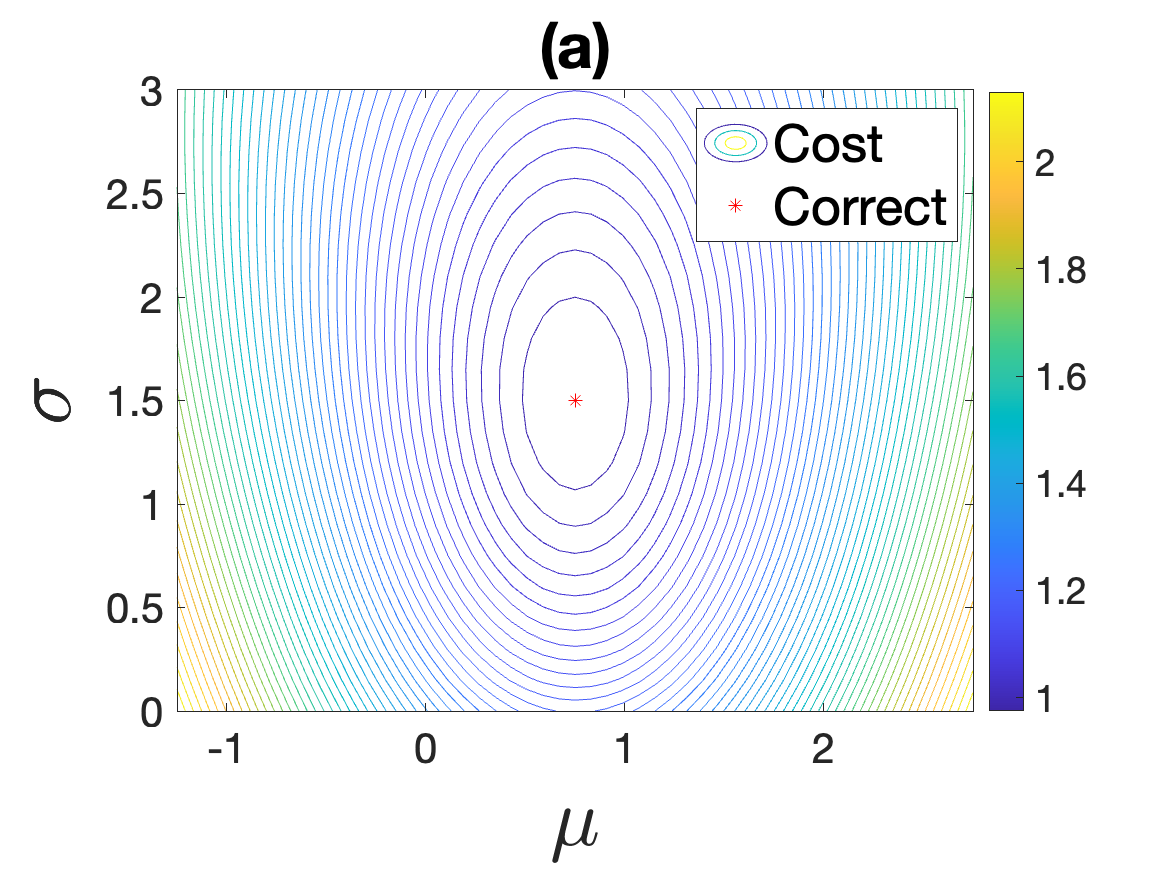
\includegraphics[width=0.245\linewidth]{figures/L1std_P2.png}
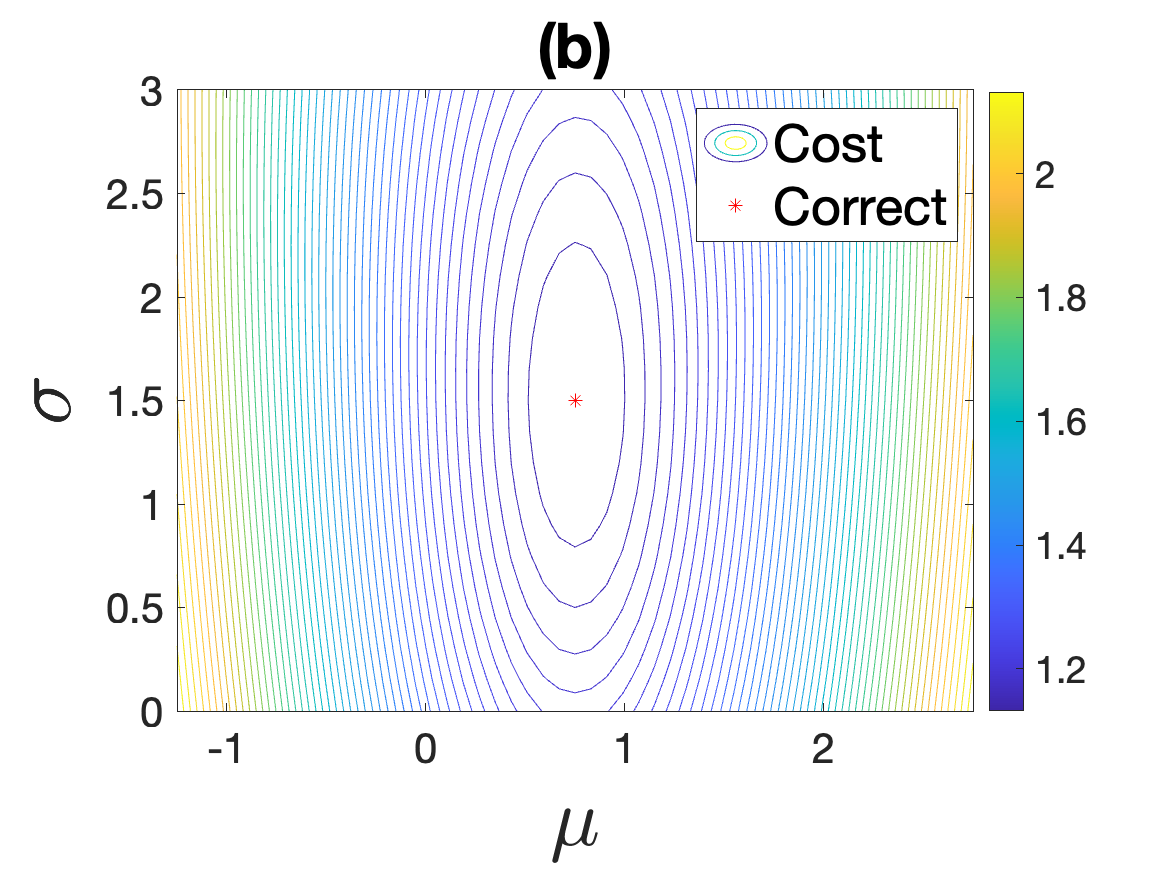
\includegraphics[width=0.245\linewidth]{figures/L1std_P8.png}
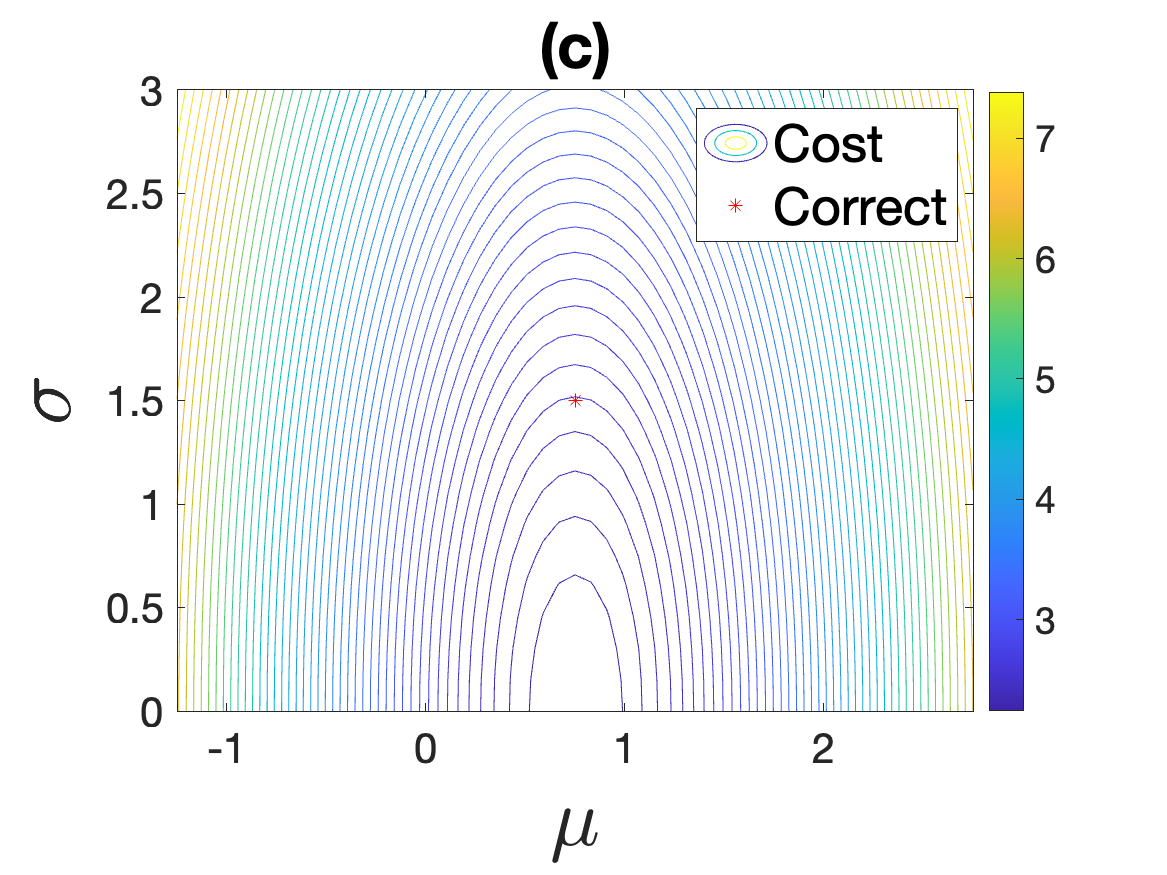
\includegraphics[width=0.245\linewidth]{figures/L2_P8.png}
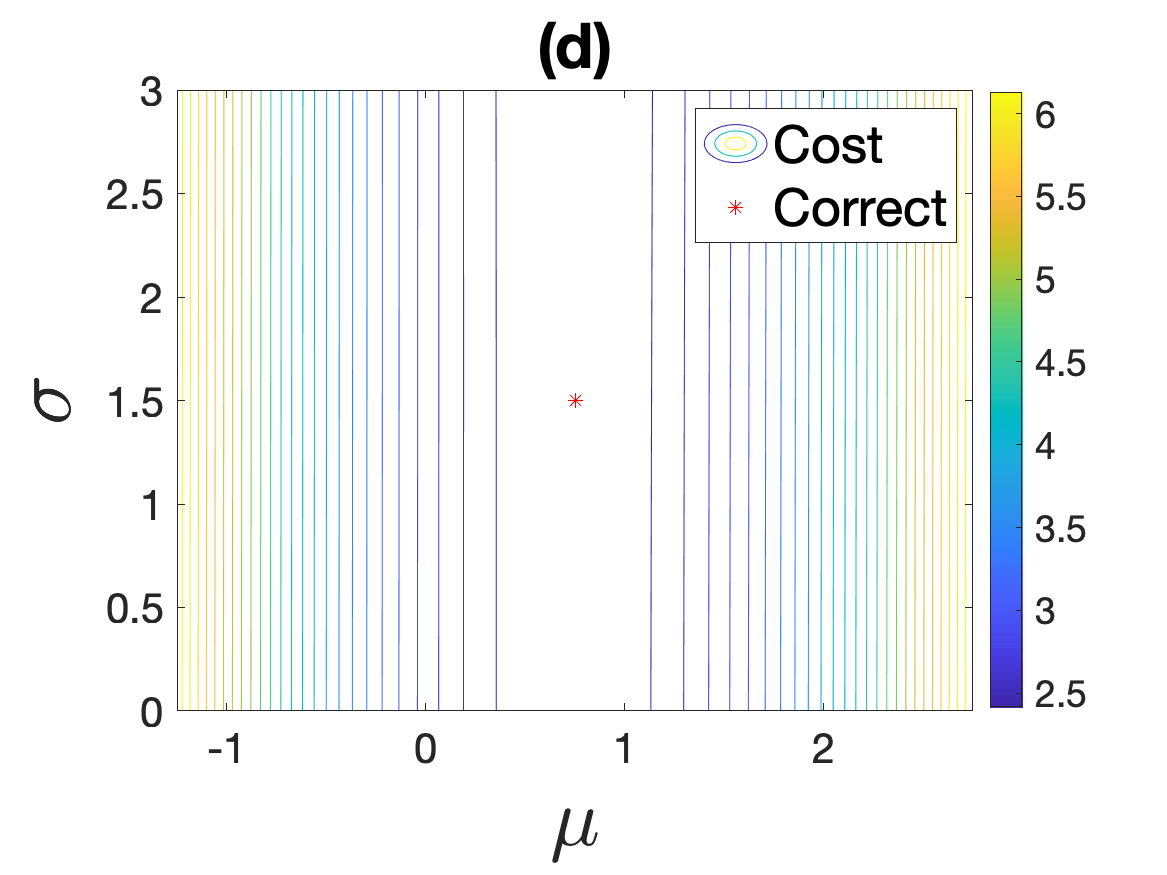
\includegraphics[width=0.245\linewidth]{figures/L2var_P8.png}\\[-3mm]
\caption{The contours show the regularizer value versus $\vec{\theta}\!=\![\mu,\sigma]\tran$ for four different regularizers:
(a) supervised-$\ell_1$ plus SD reward with $\betastd\!=\!\betastdG$ at $P\train\!=\!2$,
(b) supervised-$\ell_1$ plus SD reward with $\betastd\!=\!\betastdG$ at $P\train\!=\!8$,
(c) supervised-$\ell_2$ at $P\train\!=\!8$, 
and
(d) supervised-$\ell_2$ plus variance reward at $P\train\!=\!8$.
The red star shows the true posterior parameters $[\mu_0,\sigma_0]\tran$.
%Subplots (a)-(b) show that supervised-$\ell_1$ plus SD reward recovers the true parameters $[\mu_0,\sigma_0]\tran$ for any $P\!\geq\! 2$.
%Comparing subplots (a) and (b), a smaller $P$ yields a stronger effect.
%Subplot (c) shows that supervised-$\ell_2$ promotes mode collapse (i.e., $\hat{\sigma}\!=\!0$), while
%subplot (d) shows that adding a variance reward to supervised-$\ell_2$ discourages mode collapse but does not recover the true parameters $[\mu_0,\sigma_0]\tran$.
}
\label{fig:illustration}
\end{figure*}

We note that regularizing a cGAN with supervised-$\ell_1$ loss alone is not new; see, e.g., \cite{Isola:CVPR:17}.
%\cite{Zhao:MIA:18} ADD TO ACCEPTED PAPER
In fact, the use of supervised-$\ell_1$ loss is often preferred over $\ell_2$ in image recovery because it results in sharper, more visually pleasing results \cite{Zhao:TCI:17}. 
But regularizing a cGAN using supervised-$\ell_1$ loss \emph{alone} can push the generator towards mode collapse, for reasons described below.
%similar to the supervised-$\ell_2$ case discussed earlier.
For example, in \cite{Isola:CVPR:17}, $\ell_1$-induced mode collapse led the authors to use dropout to induce generator variation, instead of random $\vec{z}_i$.

%Our contribution is to use a properly weighted SD reward in conjunction with supervised-$\ell_1$ loss, as in \eqref{LonestdP}.
%As we show below, under certain assumptions, the SD reward works together with the $\ell_1$ loss to enforce the correctness of both the posterior mean \emph{and} the posterior covariance.
%This stands in contrast to the case of $\ell_2$ loss with a variance reward, which enforces only the correctness of the posterior mean.

\paragraph{Why not supervised-\texorpdfstring{$\ell_2$}{L2} regularization?} 
One may wonder: Why regularize using supervised-$\ell_1$ loss plus an SD reward in \eqref{LonestdP} and not a more conventional choice like supervised-$\ell_2$ loss plus a variance reward, or even supervised-$\ell_2$ loss alone?
We start by discussing the latter.

The use of supervised-$\ell_2$ regularization in a cGAN can be found in \cite{Isola:CVPR:17}.
In this case, to train the generator, one would aim to solve $\arg\min_{\vec{\theta}} \{\Ladv(\vec{\theta},\vec{\phi}) + \lambda \Ltwo(\vec{\theta})\}$ with some $\lambda>0$ and
\begin{align}
\Ltwo(\vec{\theta})
&\defn \Exy\big\{ \|\vec{x}-\Ez\{G_{\vec{\theta}}(\vec{z},\vec{y})\}\|^2_2 \big\}
\label{eq:Ltwo} .
\end{align}
Ohayon et al.~\cite{Ohayon:ICCVW:21} revived this idea for the explicit purpose of fighting mode collapse.
%They show that $\Ltwo$ regularization is consistent with the cGAN objective 
%in that, \emph{if} there exists some $\vec{\theta}$ for which $\pxhgy$ matches the true posterior $\pxgy$,
%%(recall that $\hvec{x}\defn G_{\vec{\theta}}(\vec{z},\vec{y})|_{\vec{z}\sim\pz}$)
%then both $\Ladv$ and $\Ltwo$ are minimized by the same $\vec{\theta}$.
%This is because $\Ltwo(\vec{\theta})$ is minimized when $\Ez\{G_{\vec{\theta}}(\vec{z},\vec{y})\}$ equals the MMSE estimate of $\vec{x}$ from $\vec{y}$, i.e., the posterior mean $\Exgy\{\vec{x}|\vec{y}\}$. 
%%So, both $\Ladv$ and $\Ltwo$ are minimized by the $\vec{\theta}$ for which $G_{\vec{\theta}}$ samples from the true posterior $\pxgy$, if such a $\vec{\theta}$ exists.
%In practice, such a $\vec{\theta}$ may not exist, in which case $\Ladv$ and $\Ltwo$ will act in complementary ways to drive $G_{\vec{\theta}}$ towards the true-posterior generator. 
In practice, however, the $\Ez$ term in \eqref{Ltwo} must be implemented by a finite-sample average, giving
\begin{align}
\LtwoPt(\vec{\theta})
&\defn \textstyle \ExzPy\big\{ \big\|\vec{x}-\frac{1}{P\train}\sum_{i=1}^{P\train} G_{\vec{\theta}}(\vec{z}_i,\vec{y}) \big\|^2_2 \big\} 
\label{eq:LtwoP} 
\end{align}
for some $P\train\geq 2$.
For example, Ohayon's implementation \cite{Ohayon:github:21} used $P\train=8$.
As we show in \propref{L2P}, $\LtwoPt$ \emph{induces} mode collapse rather than prevents it. 
%with the effect growing stronger as $P$ grows smaller.

\begin{proposition} \label{prop:L2P}
Say $P\train$ is finite and $\vec{\theta}$ has complete control over the $\vec{y}$-conditional mean and covariance of $\hvec{x}_i$.
Then the parameters
$\vec{\theta}_* = \arg\min_{\vec{\theta}} \LtwoPt(\vec{\theta})$ 
yield generated statistics
\begin{subequations}
\begin{align}
\Ezigy\{\hvec{x}_i(\vec{\theta}_*)|\vec{y}\} &= \Exgy\{\vec{x}|\vec{y}\} = \hvec{x}\mmse \\
\Covzigy\{\hvec{x}_i(\vec{\theta}_*)|\vec{y}\} &= \vec{0} .
\end{align}
\end{subequations}
Thus, minimizing $\LtwoPt$ encourages mode collapse.
\end{proposition}
%\begin{proof}
%See \appref{L2P}.
%\end{proof}

The proof (see \appref{L2P}) follows from the bias-variance decomposition of \eqref{LtwoP}, i.e.,
\begin{align}
&\lefteqn{\LtwoPt(\vec{\theta})}\nonumber\\
&= \textstyle \Ey\big\{ 
    \|\hvec{x}\mmse-\Ezigy\{\hvec{x}_i(\vec{\theta})|\vec{y}\}\|_2^2 
    + \tfrac{1}{P\train} 
      \tr [ \Covzigy\{\hvec{x}_i(\vec{\theta}) | \vec{y}\} ]
    + \Exgy\{\|\vec{e}\mmse\|_2^2 | \vec{y}\} 
    \big\}
\label{eq:LtwoPerrt} ,
\end{align}
where $\vec{e}\mmse\defn \vec{x}-\vec{x}\mmse$ is the MMSE error.
\Figref{illustration}(c) shows that $\LtwoPt$ regularization causes mode collapse in the toy example, and \secref{MRIexperiments} shows that it causes mode collapse in MRI. 

% REMOVING DISCUSSION OF TRAINING TIME VS P
%Experimentally, we observe that supervised-$\ell_2$ regularization does indeed lead to mode collapse when $P=2$.
%Although mode collapse may not occur with larger values of $P$, there is a high cost to using large $P$ as a result of GPU memory constraints: as $P$ doubles, the batch size must halve, and so training time increases linearly with $P$.
%For example, in our MRI experiment, we found that $P=2$ takes $\approx 2.5$ days to train for 100 epochs on a $4\times$A100 GPU server, while $P=8$ takes $\approx 10$ days.

\paragraph{Why not supervised $\ell_2$ plus a variance reward?} 
To mitigate $\LtwoPt$'s incentive for mode-collapse, the second term in \eqref{LtwoPerrt} could be canceled using a variance reward, giving 
%In particular, to train the generator, one could solve 
%\begin{align}
%\arg\min_{\vec{\theta}} \big\{ \betaadv\Ladv(\vec{\theta},\vec{\phi}) + \LtwovarP(\vec{\theta},\betavar) \big\}
%\end{align}
%with some $\betaadv,\betavar>0$ and $P\geq 2$ using
\begin{align}
% HARDWIRING \betavar = 1/P\train
\LtwovarPt(\vec{\theta})
&\defn \textstyle \LtwoPt(\vec{\theta}) - \frac{1}{P\train}\LvarPt(\vec{\theta})
\label{eq:LtwovarP} \\
\text{with~}\LvarPt(\vec{\theta})
&\defn \textstyle \frac{1}{P\train-1}\sum_{i=1}^{P\train} \EzPy\{\|\hvec{x}_i(\vec{\theta})-\hvec{x}\avgP(\vec{\theta})\|_2^2\}
\label{eq:LvarP} .
\end{align}
since \appref{LvarPerr} shows that $\LvarPt(\vec{\theta})$ is an unbiased estimator of the posterior trace-covariance:
%\eqref{LvarP} can be rewritten as
\begin{align}
\LvarPt(\vec{\theta})
%&= \textstyle \Ey\big\{ \Ezigy\{\|\vec{d}_i\|_2^2 | \vec{y}\} \big\}
&= \textstyle \Ey \{ \tr [ \Covzigy\{\hvec{x}_i(\vec{\theta}) | \vec{y}\} ] \}
\text{~~for any~} P\train\geq 2
\label{eq:LvarPerr}.
\end{align}
%with $\vec{d}_i$ from \eqref{quantities}, so that
%\begin{align}
%\LtwovarP(\vec{\theta},\betavar)
%= \textstyle \Ey\big\{ 
%    \|\hvec{x}\mmse-\ovec{x}\|_2^2
%    + \gamma\Ezigy\{\|\vec{d}_i\|_2^2 | \vec{y}\}
%    + \Exgy\{\|\vec{e}\mmse\|_2^2 | \vec{y}\} 
%    \big\}, 
%\label{eq:LtwovarPerr}
%\end{align}
%where $\gamma = \tfrac{1}{P}-\betavar$. 
However, the resulting $\LtwovarPt$ regularizer in \eqref{LtwovarP} does not encourage the generated covariance to match the \emph{true} posterior covariance, unlike the proposed $\LonestdPt$ regularizer in \eqref{LonestdP} (recall \propref{L1std}).
For the toy example, this behavior is visible in \figref{illustration}(d).

%\Figref{illustration}(c) plots $P$-sample supervised-$\ell_2$ loss $\LtwoP(\vec{\theta})$ from \eqref{LtwoP} versus $\vec{\theta}$ for $P=8$.
%The plot shows that the minimizing $\hvec{\theta}=\arg\min_{\vec{\theta}} \LtwoP(\vec{\theta})$ yields $\hat{\mu}=\mu_0$ and $\hat{\sigma}=0$, which corresponds to mode collapse.
%\Figref{illustration}(d) plots $P$-sample supervised-$\ell_2$ loss plus variance reward  $\LtwovarP(\vec{\theta},\betavar)$ from \eqref{LtwovarP} versus $\vec{\theta}$ for $\betavar=1/P$ and $P=8$. 
%This choice of $\betavar$ cancels the middle term in \eqref{LtwoPerr}, which is responsible for mode collapse.
%As can be seen in \figref{illustration}(d), $\hvec{\theta}=\arg\min_{\vec{\theta}} \LtwovarP(\vec{\theta},\betavar)$ is no longer unique, and there is no incentive for mode collapse (i.e., $\hat{\sigma}=0$) but no incentive to match the true variance (i.e., $\hat{\sigma}=\sigma_0$).
%\Figref{illustration}(a) plots $P$-sample supervised-$\ell_1$ loss plus SD reward $\LonestdP(\vec{\theta},\betastd)$ versus $\vec{\theta}$ from \eqref{LonestdP} for $\betastd=\betastdG$ from \eqref{betastdG} and $P=8$.
%The plots shows that $\hvec{\theta}=\arg\min_{\vec{\theta}} \LonestdP(\vec{\theta},\betastd)$ recovers the true parameters (i.e., $\hvec{\theta}=[\mu_0,\sigma_0]\tran$) as predicted by \propref{L1std}.
%Finally, \Figref{illustration}(b) repeats the experiment from \Figref{illustration}(c), but with $P=2$.
%The plot shows $\hvec{\theta}=[\mu_0,\sigma_0]\tran$ as predicted by \propref{L1std}.
%But, comparing \Figref{illustration}(b) to \Figref{illustration}(a), we can see that the cost surface becomes steeper for smaller $P$, i.e., the regularization becomes stronger.  
%In real-world experiments, we find that $\LonestdP(\vec{\theta},\betastd)$-regularized cGANs work best when trained with the minimum $P$, i.e., $P=2$.


\subsection{Auto-tuning of SD reward weight \texorpdfstring{$\betastd$}{betastd}} \label{sec:betastd}

\begin{figure*}
    \centering
    \footnotesize
    \def\tabwid{19.5mm}% row label spacing
    \begin{tabular}{>{\centering}p{\tabwid}
                    >{\centering}p{\tabwid}
                    >{\centering}p{\tabwid}
                    >{\centering}p{\tabwid}
                    >{\centering}p{\tabwid}
                    >{\centering}p{\tabwid}}
        $\betastd=0$ & $\betastd=\betastdG$ & $\betastd=1.2\betastdG$ & $\betastd=1.4\betastdG$ & $\betastd=1.6\betastdG$ & $\betastd=1.8\betastdG$
    \end{tabular}\\
    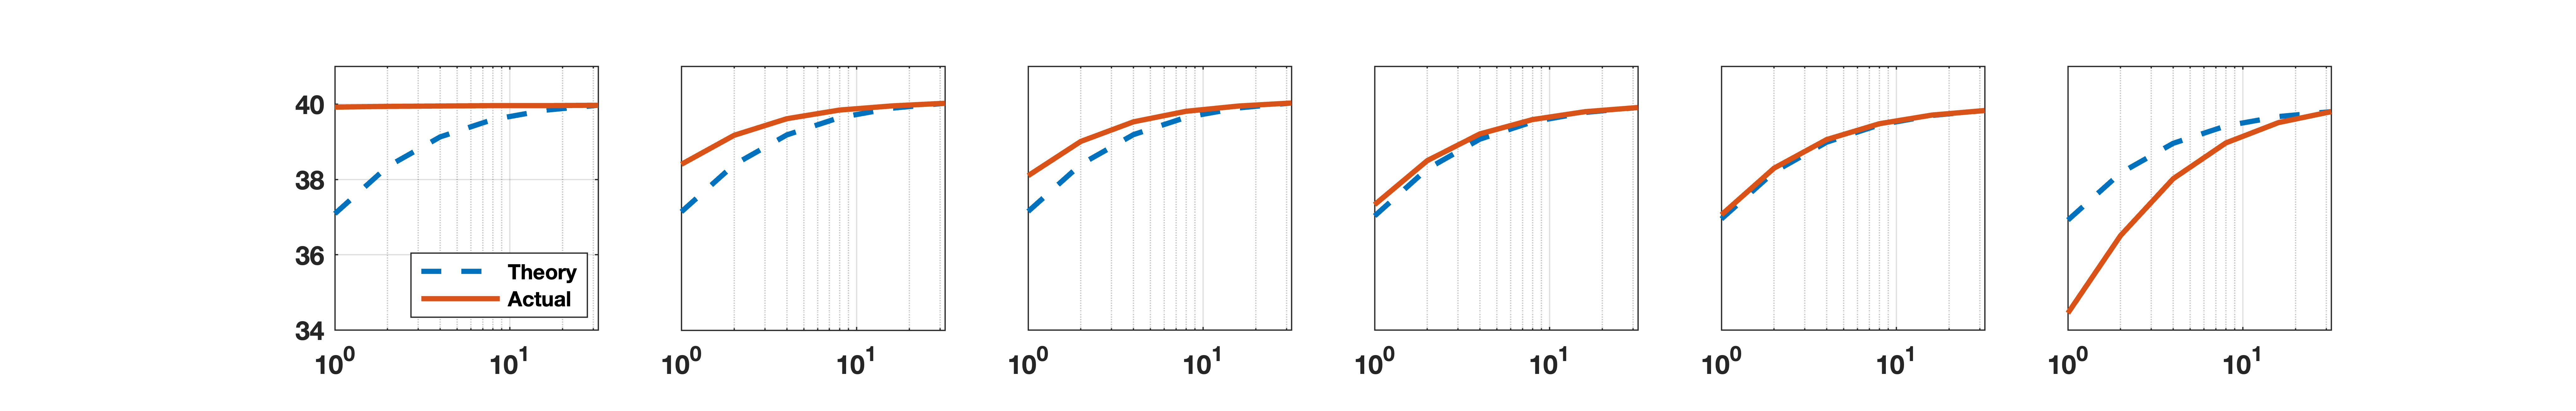
\includegraphics[width=\linewidth,trim=110 10 90 25,clip]{figures/mri/PSNR_vs_betastd_ablation.png}\\
    {\sf Number of averaged outputs, $P$, on a log scale}
    \caption{Example PSNR of $\hvec{x}\avgP$ versus $P$, the number of averaged outputs, for several training $\betastd$ and MRI recovery at $R=4$. Also shown is the theoretical behavior for true-posterior samples.}
    \label{fig:betastd_ablation}
\end{figure*}

We now propose a method to auto-tune $\betastd$ in \eqref{LonestdP} for a given training dataset.
Our approach is based on the observation that larger values of $\betastd$ tend to yield samples $\hvec{x}_i$ with more variation.
But more variation is not necessarily better; we want samples with the correct amount of variation.
To assess the correct amount of variation, we compare the expected $\ell_2$ error of the $P$-sample average $\hvec{x}\avgP$ to that of $\hvec{x}\avgone$.
%In the case of mode collapse, these errors are identical.  
When $\{\hvec{x}_i\}$ are true-posterior samples, these errors follow a particular relationship, as established by \propref{ratio} below (see \appref{ratio} for a proof).
\begin{proposition} \label{prop:ratio}
Say $\hvec{x}_i\sim \pxgy(\cdot|\vec{y})$ are independent samples of the true posterior and, for any $P\geq 1$, their $P$-sample average is $\hvec{x}\avgP\defn \frac{1}{P}\sum_{i=1}^P\hvec{x}_i$.
Then
\begin{align}
\mc{E}_P 
&\defn \E\{\|\hvec{x}\avgP-\vec{x}\|_2^2 | \vec{y}\}
= \tfrac{P+1}{P} \mc{E}\mmse 
\text{,\quad which implies\quad}
\tfrac{\mc{E}_1}{\mc{E}_P} = \tfrac{2P}{P+1} 
\label{eq:Eratio}.
\end{align}
\end{proposition}
%\begin{proof}
%See \appref{ratio}.
%\end{proof}

Experimentally we find that $\mc{E}_1/\mc{E}_P$ grows with the SD reward weight $\betastd$.
(See \figref{betastd_ablation}.)
Thus, we propose to adjust $\betastd$ so that the observed SNR-gain ratio $\mc{E}_1/\mc{E}_{P\val}$ matches the correct ratio $(2P\val)/(P\val+1)$ from \eqref{Eratio}, for some $P\val\geq 2$ that does not need to match $P\train$.
(We use $P\val=8$ in \secref{experiments}.)
In particular, at each training epoch $\tau$, we approximate $\mc{E}_{P\val}$ and $\mc{E}_1$ 
%using a validation set $\{(\vec{x}_v,\vec{y}_v)\}_{v=1}^V$ 
as follows:
\begin{align}
\hat{\mc{E}}_{P\val,\tau} 
&\defn \textstyle \frac{1}{V}\sum_{v=1}^V \|\frac{1}{P\val}\sum_{i=1}^{P\val} G_{\vec{\theta}_\tau}(\vec{z}_{i,v},\vec{y}_v)-\vec{x}_v\|_2^2 \\
\hat{\mc{E}}_{1,\tau} 
&\defn \textstyle \frac{1}{V}\sum_{v=1}^V \|G_{\vec{\theta}_\tau}(\vec{z}_{1,v},\vec{y}_v)-\vec{x}_v\|_2^2 ,
\end{align}
with validation set $\{(\vec{x}_v,\vec{y}_v)\}_{v=1}^V$ and 
i.i.d.\ codes $\{\vec{z}_{i,v}\}_{i=1}^{P\val}$.
%drawn independently of $\vec{x}_v$ and $\vec{y}_v$.
We update $\betastd$ using gradient descent:
\begin{align}
\beta_{\mathsf{SD},\tau+1}
&= \textstyle \beta_{\mathsf{SD},\tau} - \mustd \cdot \big( 
%\big[\frac{\hat{\mc{E}}_{1,\tau}}{\hat{\mc{E}}_{P\val,\tau}}\big]_{\text{dB}} 
[\hat{\mc{E}}_{1,\tau}/\hat{\mc{E}}_{P\val,\tau}]_{\text{dB}} 
%- \big[\frac{2P\val}{P\val+1}\big]_{\text{dB}} 
- [2P\val/(P\val+1)]_{\text{dB}} 
\big) \betastdG
\text{~~for~~}\tau=0,1,2,\dots
\label{eq:betastd}
\end{align}
with 
$\beta_{\mathsf{SD},0} = \betastdG$,
some $\mustd>0$, 
and $[x]_{\text{dB}}\defn 10\log_{10}(x)$.

%%%%%%%%%%%%%%%%%%%%%%%%%%%%%%%%%%%%%%%%%%%%%%%%%%%%%%%%%%%%%%%%%%%%%%%%%%%%%%%%
\section{Numerical experiments} \label{sec:experiments}
% See \url{https://github.com/matt-bendel/rcGAN}.

\subsection{Conditional Fr\'echet inception distance} \label{sec:cfid}

As previously stated, our goal is to train a generator $G_{\vec{\theta}}$ so that, for typical fixed values of $\vec{y}$, the generated distribution $\pxhgy(\cdot|\vec{y})$ matches the true posterior $\pxgy(\cdot|\vec{y})$.
It is essential to have a quantitative metric for evaluating performance with respect to this goal.
For example, it is not enough that the generated samples are ``accurate'' in the sense of being close to the ground truth, nor is it enough that they are ``diverse'' according to some heuristically chosen metric.

We quantify posterior-approximation quality using the conditional Fr\'{e}chet inception distance (CFID) \cite{Soloveitchik:21}, a computationally efficient approximation to the conditional Wasserstein distance
\begin{align}
\CWD \defn \Ey\{W_2(\pxgy(\cdot,\vec{y}),\pxhgy(\cdot,\vec{y}))\} 
\label{eq:CWD} .
\end{align}
In \eqref{CWD}, $W_2(\pa,\pb)$ denotes the Wasserstein-2 distance between distributions $\pa$ and $\pb$, defined as
\begin{align}
&W_2(\pa,\pb) 
\defn \min_{\pab\in \Pi(\pa,\pb)} \Eab\{\|\vec{a}-\vec{b}\|^2_2\} 
\label{eq:Pi} ,
\end{align}
where $\Pi(\pa,\pb) \defn \textstyle \big\{\pab : \pa=\int \pab\deriv \vec{b} \text{~and~} \pb=\int \pab \deriv \vec{a} \big\} $ denotes the set of joint distributions $\pab$ with prescribed marginals $\pa$ and $\pb$.
Similar to how FID \cite{Heusel:NIPS:17}---a popular uGAN metric---is computed, CFID approximates CWD \eqref{CWD} as follows:
i) the random vectors $\vec{x}$, $\hvec{x}$, and $\vec{y}$ are replaced by low-dimensional embeddings $\uvec{x}$, $\huvec{x}$, and $\uvec{y}$, generated by the convolutional layers of a deep network, and
ii) the embedding distributions $\pxugyu$ and $\pxuhgyu$ are approximated by multivariate Gaussians.
More details on CFID are given in \appref{cfid}.


\subsection{MRI experiments} \label{sec:MRIexperiments}
We consider parallel MRI recovery, where the goal is to recover a complex-valued multicoil image $\vec{x}$ from zero-filled measurements $\vec{y}$ (see \appref{MRI} for details).

\textbf{Data.~}
For training data $\{\vec{x}_t\}$, we used the first 8 slices of all fastMRI \cite{Zbontar:18} T2 brain training volumes with at least 8 coils, cropping to $384 \times 384$ pixels and compressing to 8 virtual coils \cite{Zhang:MRM:13}, yielding 12\,200 training images.
Using the same procedure, 2\,376 testing and 784 validation images were obtained from the fastMRI T2 brain testing volumes. 
From the 2\,376 testing images, 72 were randomly selected to evaluate the Langevin technique \cite{Jalal:NIPS:21} in order to limit its sample generation to 6 days.
%
To create the measurement $\vec{y}_t$, we transformed $\vec{x}_t$ to the Fourier domain, sampled using pseudo-random GRO patterns \cite{Joshi:22} at acceleration $R=4$ and $R=8$, and Fourier-transformed the zero-filled k-space measurements back to the (complex, multicoil) image domain.

\textbf{Architecture.~} 
We use a UNet \cite{Ronneberger:MICCAI:15} for our generator and a standard CNN for our generator, along with data-consistency as in \appref{consistency}.
Architecture and training details are given in \appref{implementation}. 

\textbf{Competitors.~} 
We compare our cGAN to the Adler and \"Oktem's cGAN \cite{Adler:18}, Ohayon et al.'s cGAN \cite{Ohayon:ICCVW:21}, Jalal et al.'s fastMRI Langevin approach \cite{Jalal:NIPS:21}, and Sriram et al.'s E2E-VarNet \cite{Sriram:MICCAI:20}.
% UNet trained to minimize the weighted combination of supervised $\ell_1$ loss and negative SSIM from \cite{Zhao:TCI:17}.
The cGAN from \cite{Adler:18} uses generator loss $\betaadv\Ladler(\vec{\theta},\vec{\phi})$ and discriminator loss $-\Ladler(\vec{\theta},\vec{\phi})+ \alpha_1 \Lgp(\vec{\phi}) + \alpha_2 \Ldrift(\vec{\phi})$, 
while the cGAN from \cite{Ohayon:ICCVW:21} uses generator loss $\betaadv\Ladv(\vec{\theta},\vec{\phi}) + \LtwoP(\vec{\theta})$ and discriminator loss $-\Ladv(\vec{\theta},\vec{\phi})+ \alpha_1 \Lgp(\vec{\phi}) + \alpha_2 \Ldrift(\vec{\phi})$.
Each used the value of $\betaadv$ specified in the original paper. 
All cGANs used the same generator and discriminator architectures, except that \cite{Adler:18} used extra discriminator input channels to facilitate the 3-input loss \eqref{Ladler}.
For the fastMRI Langevin approach \cite{Jalal:NIPS:21}, we did not modify the authors' implementation in \cite{Jalal:github:21} except to use the GRO sampling mask.
For the E2E-VarNet \cite{Sriram:MICCAI:20}, we use the same training procedure and hyperparameters outlined in \cite{Jalal:NIPS:21} except that we use the GRO sampling mask.

\textbf{Testing.~} 
To evaluate performance, we converted the multicoil outputs $\hvec{x}_i$ to complex-valued images using SENSE-based coil combining \cite{Prussmann:MRM:99} with ESPIRiT-estimated \cite{Uecker:MRM:14} coil sensitivity maps, as described in \appref{MRI}.
Magnitude images were used to compute performance metrics.
%Magnitude images were used to compute FID, CFID, APSD, PSNR, SSIM \cite{Wang:TIP:04}, LPIPS \cite{Zhang:CVPR:18}, and DISTS \cite{Ding:TPAMI:20}.
%PSNR and SSIM were computed from the $P$-averaged outputs $\hvec{x}\avgP$ (recall \eqref{quantities}), while FID and CFID were computed from the un-averaged outputs $\hvec{x}_i$.

% TABLES W/ MODELS SAVED ACCORDING TO CFID

\begin{table*}[h]
  \caption{Average MRI results at $R\in\{4,8\}$. 
    %$\pm$ shows standard error. 
    %(C)FID$^1$, PSNR, SSIM, and APSD used $72$ test samples and $P\!=\!32$. 
    CFID$^1$, FID, and APSD used $72$ test samples and $P\!=\!32$, 
    CFID$^2$ used $2\,376$ test samples and $P\!=\!8$, and 
    CFID$^3$ used all $14\,576$ samples and $P\!=\!1$}
  \vspace{0.1in}
  \label{tab:mriresults}
  \centering
  \resizebox{\textwidth}{!}{%
  \begin{tabular}{llllllllllllll}
    \toprule
    & \multicolumn{6}{c}{$R=4$} & \multicolumn{6}{c}{$R=8$}\\
    \cmidrule(lr){2-7} \cmidrule(lr){8-13}
    Model & 
    CFID$^1\!\!\downarrow$ & CFID$^2\!\!\downarrow$ & CFID$^3\!\!\downarrow$ & FID$\downarrow$ & APSD & Time (4)$\downarrow$ &
    CFID$^1\!\!\downarrow$ & CFID$^2\!\!\downarrow$ & CFID$^3\!\!\downarrow$ & FID$\downarrow$ & APSD & Time (4)$\downarrow$ \\
    \midrule
    E2E-VarNet (Sriram et al.\ \cite{Sriram:MICCAI:20}) 
        & 7.47 & 6.99 & 6.61 & 8.84 & 0.0 & 310ms 
        & 7.82 & 6.81 & 6.31 & 8.40 & 0.0 & 316ms\\
    Langevin (Jalal et al.\ \cite{Jalal:NIPS:21}) 
        & 5.29 & - & - & 6.12 & 5.9e-6 & 14 min
        & 7.34 & - & - & 14.32  & 7.6e-6 & 14 min\\
    cGAN (Adler \& \"Oktem \cite{Adler:18}) 
        & 6.39 & 4.27 & 3.82 & 5.25 & 3.9e-6 & \textbf{217 ms}
        & 10.10 & 6.30 & 5.72 & 10.77  & 7.7e-6 & \textbf{217 ms}\\
    cGAN (Ohayon et al.\ \cite{Ohayon:ICCVW:21}) 
        & 4.06 & 3.27 & 2.95 & 6.45 & 7.2e-8 & \textbf{217 ms}
        & 6.04 & 4.59 & 4.27 & 11.05  & 7.7e-7 & \textbf{217 ms}\\
    cGAN (Ours) & \textbf{3.10} 
        & \textbf{1.54} & \textbf{1.29} & \textbf{3.75} & 3.8e-6 & \textbf{217 ms}
        & \textbf{4.87} & \textbf{2.23} & \textbf{1.79} & \textbf{7.72}  & 7.6e-6 & \textbf{217 ms}\\
    \bottomrule
  \end{tabular}%
  }
\end{table*}


\textbf{Results.~} 
\tabref{mriresults} shows CFID, FID, APSD $\defn(\frac{1}{NP}\sum_{i=1}^{P} \|\hvec{x}\avgP-\hvec{x}_i\|^2)^{1/2}$, and 4-sample generation time at $R\in\{4,8\}$.
(C)FID was computed using VGG-16 (not Inception-v3) to better align with radiologists' perceptions \cite{Kastryulin:22}.
%The Langevin competitor \cite{Jalal:NIPS:21} was evaluated using only 72 test images due to its slow sample generation time (6 days).
As previously described, the Langevin method was evaluated using only 72 test images.
Because CFID is biased at small sample sizes \cite{Soloveitchik:21}, we re-evaluated the other methods using all $2\,376$ test images, and again using all $14\,576$ training and test images. 
\tabref{mriresults} shows that our approach gave significantly better CFID and FID than the competitors.
%It also gave the highest PSNR and SSIM, although SSIM was within one standard error of that from Ohayon et al\.'s cGAN.
%Although we don't consider APSD as a performance metric, we note that 
Also, the APSD of Ohayon et al.'s cGAN was an order-of-magnitude smaller than the others, indicating mode collapse.
%The small-sample bias of CFID is visible in \tabref{mriresults}, and \appref{CFID} demonstrates that it is due mainly to the covariance component of CFID.
The cGANs generated samples $3\,800$ times faster than the Langevin approach from \cite{Jalal:NIPS:21}.
%CFID and FID results at acceleration $R=4$, presented in \appref{additionalresults}, show similar trends. 

Tables \ref{tab:versusPr4} and \ref{tab:versusPr8} show PSNR, SSIM, LPIPS \cite{Zhang:CVPR:18}, and DISTS \cite{Ding:TPAMI:20} for the $P$-sample average $\hvec{x}\avgP$ at $P\in\{1,2,4,8,16,32\}$ and $R\in\{4,8\}$, respectively.
While the E2E-VarNet achieves the best PSNR at $R\in\{4,8\}$ and the best SSIM at $R=4$, the proposed cGAN achieves the best LPIPS and DISTS performances at $R\in\{4,8\}$ when $P=2$ and the best SSIM at $R=8$ when $P=8$. 
The $P$ dependence can be explained by the perception-distortion tradeoff \cite{Blau:CVPR:18}: as $P$ increases, $\hvec{x}\avgP$ transitions from better perceptual quality to lower $\ell_2$ distortion. 
PSNR favors $P\rightarrow\infty$ (e.g., $\ell_2$ optimality) while the other metrics favor particular combinations of perceptual quality and distortion.
The plots in Appendices~\ref{app:mriplotsR4} and \ref{app:mriplotsR8} show zoomed-in versions of $\hvec{x}\avgP$ that visually demonstrate the perception-distortion tradeoff at $P\in\{1,2,4,32\}$: smaller $P$ yield sharper images with more variability from the ground truth, while larger $P$ yield smoother reconstructions. 

\begin{table*}[t]
  % \color{blue}
  \caption{Average PSNR, SSIM, LPIPS, and DISTS of $\hvec{x}\avgP$ versus $P$ for $R=4$ MRI}
  \vspace{0.1in}
  \label{tab:versusPr4}
  \centering
  \resizebox{1.0\textwidth}{!}{%
  \begin{tabular}{lcccccccccccc}
    \toprule
    & \multicolumn{6}{c}{PSNR$\uparrow$} 
        & \multicolumn{6}{c}{SSIM$\uparrow$}\\ 
    \cmidrule(lr){2-7} \cmidrule(lr){8-13}
    Model & $P\!=$1 & $P\!=$2 & $P\!=$4 & $P\!=$8 & $P\!=$16 & $P\!=$32
          & $P\!=$1 & $P\!=$2 & $P\!=$4 & $P\!=$8 & $P\!=$16 & $P\!=$32\\
    \midrule
    E2E-VarNet (Sriram et al. \cite{Sriram:MICCAI:20}) & \bf 39.93 & - & - & - & - & - & \bf 0.9641 & - & - & - & - & -\\
    Langevin (Jalal et al. \cite{Jalal:NIPS:21}) 
          & 36.04 & 37.02 & 37.65 & 37.99 & 38.17 & 38.27 &  0.8989 & 0.9138 & 0.9218 & 0.9260 & 0.9281 & 0.9292\\
    cGAN (Adler \& \"Oktem \cite{Adler:18}) 
          & 35.63 & 36.64 & 37.24 & 37.56 & 37.73 & 37.82 &  0.9330 & 0.9445 & 0.9478 & 0.9480 & 0.9477 & 0.9473\\
    cGAN (Ohayon et al. \cite{Ohayon:ICCVW:21}) 
          & 39.44 & 39.46 & 39.46 & 39.47 & 39.47 & 39.47 &  0.9558 & 0.9546 & 0.9539 & 0.9535 & 0.9533 & 0.9532\\
    cGAN (Ours) 
          & 36.96 & 38.14 & 38.84 & 39.24 & 39.44 & 39.55 &  0.9440 & 0.9526 & 0.9544 & 0.9542 & 0.9537 & 0.9533\\
    & \multicolumn{6}{c}{LPIPS$\downarrow$} 
        & \multicolumn{6}{c}{DISTS$\downarrow$}\\ 
    \cmidrule(lr){2-7} \cmidrule(lr){8-13}
    Model & $P\!=$1 & $P\!=$2 & $P\!=$4 & $P\!=$8 & $P\!=$16 & $P\!=$32
          & $P\!=$1 & $P\!=$2 & $P\!=$4 & $P\!=$8 & $P\!=$16 & $P\!=$32\\
    \midrule
    E2E-VarNet (Sriram et al. \cite{Sriram:MICCAI:20}) & 0.0316 & - & - & - & - & - & 0.0859 & - & - & - & - & -\\
    Langevin (Jalal et al. \cite{Jalal:NIPS:21}) 
          & 0.0545 & 0.0394 & 0.0336 & 0.0320 & 0.0317 & 0.0316 &  0.1116 & 0.0921 & 0.0828 & 0.0793 & 0.0781 & 0.0777\\
    cGAN (Adler \& \"Oktem \cite{Adler:18}) 
          & 0.0285 & 0.0255 & 0.0273 & 0.0298 & 0.0316 & 0.0327 &  0.0972 & 0.0857 & 0.0878 & 0.0930 & 0.0967 & 0.0990\\
    cGAN (Ohayon et al. \cite{Ohayon:ICCVW:21}) 
          & 0.0245 & 0.0247 & 0.0248 & 0.0249 & 0.0249 & 0.0249 &  0.0767 & 0.0790 & 0.0801 & 0.0807 & 0.0810 & 0.0811\\
    cGAN (Ours) 
          & 0.0175 & \bf 0.0164 & 0.0188 & 0.0216 & 0.0235 & 0.0245 &  \bf 0.0546 & 0.0563 & 0.0667 & 0.0755 & 0.0809 & 0.0837\\
    \bottomrule
  \end{tabular}%
  }
\end{table*}


\begin{table*}[t]
  \caption{Average PSNR, SSIM, LPIPS, and DISTS of $\hvec{x}\avgP$ versus $P$ for $R=8$ MRI}
  \vspace{0.1in}
  \label{tab:versusPr8}
  \centering
  \resizebox{1.0\textwidth}{!}{%
  \begin{tabular}{lcccccccccccc}
    \toprule
    & \multicolumn{6}{c}{PSNR$\uparrow$} 
        & \multicolumn{6}{c}{SSIM$\uparrow$}\\ 
    \cmidrule(lr){2-7} \cmidrule(lr){8-13}
    Model & $P\!=$1 & $P\!=$2 & $P\!=$4 & $P\!=$8 & $P\!=$16 & $P\!=$32
          & $P\!=$1 & $P\!=$2 & $P\!=$4 & $P\!=$8 & $P\!=$16 & $P\!=$32\\
    \midrule
    E2E-VarNet (Sriram et al.\ \cite{Sriram:MICCAI:20}) & \bf 36.49 & - & - & - & - & - & 0.9220 & - & - & - & - & -\\
    % UNet & 34.77 & 34.77 & 34.77 & 34.77 & 34.77 & 34.77 
          % & 0.9228 & 0.9228 & 0.9228 & 0.9228 & 0.9228 & 0.9228\\
    Langevin (Jalal et al. \cite{Jalal:NIPS:21}) 
          & 32.17 & 32.83 & 33.45 & 33.74 & 33.83 & 33.90
          & 0.8725 & 0.8919 & 0.9031 & 0.9091 & 0.9120 & 0.9137\\
    cGAN (Adler \& \"Oktem \cite{Adler:18}) 
          & 31.31 & 32.31 & 32.92 & 33.26 & 33.42 & 33.51
          & 0.8865 & 0.9045 & 0.9103 & 0.9111 & 0.9102 & 0.9095\\
    cGAN (Ohayon et al. \cite{Ohayon:ICCVW:21}) 
          & 34.89 & 34.90 & 34.90 & 34.90 & 34.91 & 34.92
          & 0.9222 & 0.9217 & 0.9213 & 0.9211 & 0.9211 & 0.9210\\
    cGAN (Ours) 
          & 32.32 & 33.67 & 34.53 & 35.01 & 35.27 & 35.42
          & 0.9030 & 0.9199 & 0.9252 & \bf 0.9257 & 0.9251 & 0.9246\\
    & \multicolumn{6}{c}{LPIPS$\downarrow$} 
        & \multicolumn{6}{c}{DISTS$\downarrow$}\\ 
    \cmidrule(lr){2-7} \cmidrule(lr){8-13}
    Model & $P\!=$1 & $P\!=$2 & $P\!=$4 & $P\!=$8 & $P\!=$16 & $P\!=$32
          & $P\!=$1 & $P\!=$2 & $P\!=$4 & $P\!=$8 & $P\!=$16 & $P\!=$32\\
    \midrule
    E2E-VarNet (Sriram et al.\ \cite{Sriram:MICCAI:20}) & 0.0575 & - & - & - & - & - & 0.1253 & - & - & - & - & -\\
    % UNet & 0.0586 & 0.0586 & 0.0586 & 0.0586 & 0.0586 & 0.0586
          % & 0.1120 & 0.1120 & 0.1120 & 0.1120 & 0.1120 & 0.1120\\
    Langevin (Jalal et al. \cite{Jalal:NIPS:21}) 
          & 0.0769 & 0.0619 & 0.0579 & 0.0589 & 0.0611 & 0.0611
          & 0.1341 & 0.1136 & 0.1086 & 0.1119 & 0.1175 & 0.1212\\
    cGAN (Adler \& \"Oktem \cite{Adler:18}) 
          & 0.0698 & 0.0614 & 0.0623 & 0.0667 & 0.0704 & 0.0727
          & 0.1407 & 0.1262 & 0.1252 & 0.1291 & 0.1334 & 0.1361\\
    cGAN (Ohayon et al. \cite{Ohayon:ICCVW:21}) 
          & 0.0532 & 0.0536 & 0.0539 & 0.0540 & 0.0534 & 0.0540
          & 0.1128 & 0.1143 & 0.1151 & 0.1155 & 0.1157 & 0.1158\\
    cGAN (Ours) 
          & 0.0418 & \bf 0.0379 & 0.0421 & 0.0476 & 0.0516 & 0.0539
          & 0.0906 & \bf 0.0877 & 0.0965 & 0.1063 & 0.1135 & 0.1177\\
    \bottomrule
  \end{tabular}%
  }
\end{table*}

\newcommand{\MRIavgsampsamp}[7]{
    \begin{figure}[t]
    \def\tabwidcol{21mm} % row label spacing
    \def\tabwidrow{21mm} % row label spacing
    \def\figwid{0.18\columnwidth}
    \def\figheight{0.54\columnwidth}
    \hspace{10mm}
    \hspace{\figwid}
    %\rotatebox{0}
        {\sf \scriptsize
        \begin{tabular}{>{\centering}p{\tabwidrow}>{\centering}p{\tabwidrow}>{\centering}p{\tabwidrow}>{\centering}p{\tabwidrow}}
        cGAN (ours) & cGAN (Ohayon) & cGAN (Adler) & Langevin (Jalal)
        \end{tabular}}\\[-0.5mm]
    \rotatebox{90}{\sf \scriptsize
        \begin{tabular}{>{\centering}p{\tabwidcol}>{\centering}p{\tabwidcol}>{\centering}p{\tabwidcol}}
        E2E-VarNet & Truth & Truth
        \end{tabular}}%
    \begin{tikzpicture}
        \node[anchor=south west,inner sep=0] at (0,0) {\includegraphics[height=\figheight,trim=10 10 5 10,clip]{figures/mri/body_figs/body_mri_fig_R_#7_left_#1.png}};
        \draw [-latex, line width=1pt, yellow] (#2,\fpeval{#3 + #6}) -- (#4,\fpeval{#5 + #6});
        \draw [-latex, line width=1pt, yellow] (#2,#3) -- (#4,#5);
    \end{tikzpicture}
    % \includegraphics[height=\figheight,trim=10 10 5 10,clip]{figures/mri/body_figs/body_mri_fig_left_#1.png}
    \hspace{2mm}
    \rotatebox{90}{\sf \scriptsize
        \begin{tabular}{>{\centering}p{\tabwidcol}>{\centering}p{\tabwidcol}>{\centering}p{\tabwidcol}}
        Sample & Sample & Average (P=32)
        \end{tabular}}%
    \begin{tikzpicture}
        \node[anchor=south west,inner sep=0] at (0,0) {\includegraphics[height=\figheight,trim=10 10 5 10,clip]{figures/mri/body_figs/body_mri_fig_R_#7_right_#1.png}};
        % Our samps
        \draw [-latex, line width=1pt, yellow] (#2,\fpeval{#3 + 2*#6}) -- (#4,\fpeval{#5 + 2*#6});
        \draw [-latex, line width=1pt, yellow] (#2,\fpeval{#3 + #6}) -- (#4,\fpeval{#5 + #6});
        \draw [-latex, line width=1pt, yellow] (#2,#3) -- (#4,#5);

        % Ohayon samps
        \draw [-latex, line width=1pt, yellow] (\fpeval{#2 + #6},\fpeval{#3 + 2*#6}) -- (\fpeval{#4 + #6},\fpeval{#5 + 2*#6});
        \draw [-latex, line width=1pt, yellow] (\fpeval{#2 + #6},\fpeval{#3 + #6}) -- (\fpeval{#4 + #6},\fpeval{#5 + #6});
        \draw [-latex, line width=1pt, yellow] (\fpeval{#2 + #6},#3) -- (\fpeval{#4 + #6},#5);

        % Adler samps
        \draw [-latex, line width=1pt, yellow] (\fpeval{#2 + 2*#6},\fpeval{#3 + 2*#6}) -- (\fpeval{#4 + 2*#6},\fpeval{#5 + 2*#6});
        \draw [-latex, line width=1pt, yellow] (\fpeval{#2 + 2*#6},\fpeval{#3 + #6}) -- (\fpeval{#4 + 2*#6},\fpeval{#5 + #6});
        \draw [-latex, line width=1pt, yellow] (\fpeval{#2 + 2*#6},#3) -- (\fpeval{#4 + 2*#6},#5);

        % Langevin samps
        \draw [-latex, line width=1pt, yellow] (\fpeval{#2 + 3*#6},\fpeval{#3 + 2*#6}) -- (\fpeval{#4 + 3*#6},\fpeval{#5 + 2*#6});
        \draw [-latex, line width=1pt, yellow] (\fpeval{#2 + 3*#6},\fpeval{#3 + #6}) -- (\fpeval{#4 + 3*#6},\fpeval{#5 + #6});
        \draw [-latex, line width=1pt, yellow] (\fpeval{#2 + 3*#6},#3) -- (\fpeval{#4 + 3*#6},#5);
        % 4.45 -> 6.65 (corner to corner)
    \end{tikzpicture}
    \caption{Example $R=#7$ MRI reconstructions. Arrows show meaningful variations across samples.}
    \label{fig:avgsampsamp_#1}
    \end{figure}
}

\newcommand{\MRIavgerrstd}[2]{
    \begin{figure}[t]
    \def\tabwidcol{21mm} % row label spacing
    \def\tabwidrow{19mm} % row label spacing
    \def\figwid{0.18\columnwidth}
    \rotatebox{0}{\sf \scriptsize
        \begin{tabular}{>{\centering}p{\tabwidrow}>{\centering}p{\tabwidrow}>{\centering}p{\tabwidrow}>{\centering}p{\tabwidrow}>{\centering}p{\tabwidrow}>{\centering}p{\tabwidrow}}
        Truth & E2E-VarNet & cGAN (ours) & cGAN (Ohayon) & cGAN (Adler) & Langevin (Jalal)
        \end{tabular}
    }
    \\
    \includegraphics[width=\columnwidth,trim=10 10 10 10,clip]{figures/mri/body_figs/body_mri_fig_R_#2_avg_err_std_#1.png}
    \caption{Example $R=#2$ MRI reconstructions with $P=32$. 
    Row one: $P$-sample average $\hvec{x}\avgP$. 
    Row two: pixel-wise absolute error $|\hvec{x}\avgP-\vec{x}|$.
    Row three: pixel-wise SD $(\frac{1}{P}\sum_{i=1}^P(\hvec{x}_i-\hvec{x}\avgP)^2)^{1/2}$.}
    \label{fig:avgerrstd_#1}
    \end{figure}
}

\MRIavgsampsamp{19}{2.0}{1.65}{1.5}{1.5}{2.55}{8}
\MRIavgerrstd{19}{8}

\Figref{avgsampsamp_19} shows zoomed versions of two posterior samples $\hvec{x}_i$, as well as $\hvec{x}\avgP$, at $P=32$ and $R=8$.
The posterior samples show meaningful variations for the proposed method, essentially no variation for Ohayon et al.'s cGAN, and vertical or horizontal reconstruction artifacts for Adler \& \"Oktem's cGAN and the Langevin method, respectively.
The $\hvec{x}\avgP$ plots show that these artifacts are mostly suppressed by sample averaging with large $P$.
%Our approach produces sharp samples with realistic variation (indicated by the arrows), whereas Adler \& \"Oktem's cGAN produces samples that have vertical strip artifacts, while the Langevin technique produces samples with horizontal stripe artifacts.

\Figref{avgerrstd_19} shows examples of $\hvec{x}\avgP$, along with the corresponding pixel-wise absolute errors $|\hvec{x}\avgP-\vec{x}|$ and pixel-wise SD images $(\frac{1}{P}\sum_{i=1}^P (\hvec{x}\avgP-\hvec{x}_i)^2)^{1/2}$, for $P=32$ and $R=8$.
The absolute-error image for the Langevin technique looks more diffuse than those of the other methods in the brain region.
The fact that it is brighter in the air region (i.e., near the edges) is a consequence of minor differences in sensitivity-map estimation.
The pixel-wise SD images show a lack of variability for the E2E-VarNet, which does not generate posterior samples, as well as Ohayon et al.'s cGAN, due to mode collapse.
The Langevin pixel-wise SD images show localized hot-spots that appear to be reconstruction artifacts. 

Appendices \ref{app:mriplotsR4} and \ref{app:mriplotsR8} show other example MRI recoveries with zoomed pixel-wise SD images at $R=4$ and $R=8$, respectively. 
Notably, Figures \ref{fig:mriapp_11} and \ref{fig:mriapp_9} show strong hallucinations for Langevin recovery at $R=8$, as highlighted by the red arrows.

\subsection{Inpainting experiments} \label{sec:inpainting}
In this section, our goal is to complete a large missing square in a face image.

\textbf{Data.~}
We used $256 \times 256$ CelebA-HQ face images \cite{Karras:ICLR:18} and a centered $128\times 128$ missing square.
We randomly split the dataset, yielding $27\,000$ training, $2\,000$ validation, and $1\,000$ testing images. 

\textbf{Architecture.~} 
For our cGAN, we use the CoModGAN generator and discriminator from \cite{Zhao:ICLR:21} with our proposed $\LonestdPt$ regularization. Unlike \cite{Zhao:ICLR:21}, we do not use MBSD \cite{Karras:ICLR:18} at the discriminator.

\begin{table*}[t]
  \caption{Average results for inpainting:
  FID was 
  computed from $1\,000$ test images with $P\!=\!32$,
  while CFID was computed from all 30\,000 images with $P\!=\!1$}
  \label{tab:inpainting256}
  \centering
  \vspace{0.1in}
  \resizebox{0.6\columnwidth}{!}{%
  \begin{tabular}{llll}
    \toprule
    Model & CFID$\downarrow$ & FID$\downarrow$ 
        %& PSNR$\uparrow$ & SSIM$\uparrow$ 
        & Time (128)$\downarrow$\\
    \midrule
    Score-SDE (Song et al.\ \cite{Song:ICLR:21}) & 5.11 & 7.92 
        %& 26.11 $\pm$ 0.09 & 0.9025 $\pm$ 0.0007 
        & 48 min\\
    CoModGAN (Zhao et al.\ \cite{Zhao:ICLR:21}) & 5.29 & 8.50 
        %& 25.45 $\pm$ 0.06 & 0.8882 $\pm$ 0.0006 
        & \textbf{217 ms}\\
    cGAN (ours) & \textbf{4.69} & \textbf{7.45} 
        %& \textbf{26.61} $\pm$ 0.07 & \textbf{0.9037} $\pm$ 0.0007 
        & \textbf{217 ms}\\
    \bottomrule
  \end{tabular}%
  }
\end{table*}

\textbf{Training/validation/testing.~}
We use the same general training and testing procedure described in \secref{MRIexperiments}, but with $\betaadv=$ 5e-3, $n\batch=100$, and 110 epochs of cGAN training.
Running PyTorch on a server with 4 Tesla A100 GPUs, each with 82~GB of memory, the cGAN training takes approximately 2 days.
FID was evaluated on $1\,000$ test images using $P\!=\!32$ samples per measurement.
To avoid the bias that would result from evaluating CFID on only $1\,000$ images (see \appref{CFID}), CFID was evaluated on all $30\,000$ images with $P=1$. 

\textbf{Competitors.~} 
We compare with the state-of-the-art CoModGAN \cite{Zhao:ICLR:21}
and Score-based SDE \cite{Song:ICLR:21} approaches.
For CoModGAN, we use the PyTorch implementation from \cite{Zeng:github:22}. 
CoModGAN differs from our cGAN only in its use of MBSD and lack of $\LonestdPt$ regularization.
For Song et al.'s SDE, we use the authors' implementation from \cite{Song:github:21b} with their pretrained weights and the settings they suggested for the $256\times256$ CelebA-HQ dataset.

\textbf{Results.~} 
\tabref{inpainting256} shows test CFID, FID, and 128-sample generation time.
The table shows that our approach gave the best CFID and FID, and that the cGANs generated samples 13\,000 times faster than the score-based method.
\Figref{inpainting_22} shows an example of five generated samples for the three methods under test. 
The samples are all quite good, although a few generated by CoModGAN and the score-based technique have minor artifacts.  
Some samples generated by our technique show almond-shaped eyes, demonstrating fairness.
Additional examples are given in \appref{inpaintingplots}.

\newcommand{\inpaintingFigRow}[2]{
    \def\fighgt{21mm}
    \begin{figure}[#2]
    \centering
    {\scriptsize\sf
    \rotatebox{90}{\hspace{6mm} Original}%
        \includegraphics[height=\fighgt]{figures/inpainting/original_#1.png}
    \hspace{3mm}
    \rotatebox{90}{\hspace{1mm} \textcolor{white}{Sg}cGAN (ours)\textcolor{white}{N}}\,%
        \includegraphics[height=\fighgt,trim=10 9 10 6,clip]
            {figures/inpainting/5_recons_ours_#1.png}\\[0mm]
    \rotatebox{90}{\hspace{3mm} \textcolor{white}{Sg}Masked\textcolor{white}{N}}%
        \includegraphics[height=\fighgt]{figures/inpainting/masked_#1.png}
    \hspace{3mm}
    \rotatebox{90}{\hspace{0mm} \textcolor{white}{Sg}CoModGAN \textcolor{white}{N}}\,%
        \includegraphics[height=\fighgt,trim=10 9 10 6,clip]
            {figures/inpainting/5_recons_comodgan_#1.png}\\[0mm]
    \hspace{7mm}\hspace{\fighgt}
    \rotatebox{90}{\hspace{0mm} \textcolor{white}{Sg}Score-SDE\textcolor{white}{N}}\,%
        \includegraphics[height=\fighgt,trim=10 9 10 6,clip]
            {figures/inpainting/5_recons_langevin_#1.png}}
    \vspace{-2mm}
    \caption{Example of inpainting a $128\!\times\!128$ square on a $256\!\times\!256$ resolution CelebA-HQ image.}
    \label{fig:inpainting_#1}
\end{figure}
}

\inpaintingFigRow{22}{t}

%------------------------------------------------------------------------
\section{Conclusion} \label{sec:conclusion}
We propose a novel regularization framework for image-recovery cGANs that consists of supervised-$\ell_1$ loss plus an appropriately weighted standard-deviation reward.
%, i.e., $\LoneP(\vec{\theta}) - \betastd\LstdP(\vec{\theta})$. 
For the case of an independent Gaussian posterior, we proved that our regularization yields generated samples that agree with the true-posterior samples in both mean and covariance.
We also established limitations for alternatives based on supervised-$\ell_2$ regularization with or without a variance reward.
For practical datasets, we proposed a method to auto-tune our standard-deviation reward weight.

Experiments on parallel MRI and large-scale face inpainting showed our proposed method outperforming all cGAN and score-based competitors in CFID, which measures posterior-approximation quality, as well as other metrics like FID, PSNR, SSIM, LPIPS, and DISTS.
Furthermore, it generates samples thousands of times faster than Langevin/score-based approaches.

% \textr{[MB: Moved this up here to separate it from the limitations. I know that the first sentence is a limitation, but I feel like flows better here since the final thought directly combats it. Then, the subsequent limitations section focuses on limitations which are more general (i.e., clinical studies needed to validate results, ImageNet features)]}
% In our current implementation, our cGAN is trained for a specific image-recovery task and may not generalize to new tasks. \textr{[MB: I think we implicitly acknowledge this in the following sentence.]}
In ongoing work, we are extending our approach so that it can be trained to handle a wide range of recovery tasks, such as MRI with a generic acceleration and sampling mask \cite{Bendel:NIPSW:23}, or inpainting with a generic mask.
%In the inpainting and MR applications, for example, our generator could take in both the measurements $\vec{y}$ and the sampling mask.
We are also extending our approach to other applications, such as super-resolution, deblurring, compressive sensing, denoising, and phase retrieval.

\textbf{Limitations.~} 
We acknowledge several limitations of our work.
First, while our current work focuses on how to build a fast and accurate posterior sampler, it's not yet clear how to best exploit the resulting posterior samples in each given application.
For example, in MRI, where the posterior distribution has the potential to help assess uncertainty in image recovery, it's still not quite clear how to best convey uncertainty information to radiologists (e.g., they may not gain much from pixel-wise SD images).
More work is needed on this front.
Second, we acknowledge that, because radiologists are risk-averse, more studies are needed before they will feel comfortable incorporating generative deep-learning-based methods into the clinical workflow.
Third, we acknowledge that the visual quality of our $R=8$ MRI reconstructions falls below clinical standards.
Fourth, some caution is needed when interpreting our CFID, FID, and DISTS perceptual metrics because the VGG-16 backbone used to compute them was trained on ImageNet data. 
Although there is some evidence that the resulting DISTS metric correlates well with radiologists' perceptions \cite{Kastryulin:22}, there is also evidence that ImageNet-trained features may discard information that is diagnostically relevant in medical imaging \cite{Kynkaanniemi:22}.
Thus our results need to be validated with a pathology-centric radiologist study before they can be considered relevant to clinical practice.


%%%%%%%%%%%%%%%%%%%%%%%%%%%%%%%%%%%%%%%%%%%%%%%%%%%%%%%%%%%%%%%%%%%%%%%%%%%%%%%%
\begin{ack}
The authors are funded in part by the National Institutes of Health under grant R01-EB029957 and the National Science Foundation under grant CCF-1955587. 
\end{ack}

\bibliographystyle{ieeetr}
\small
\bibliography{macros_abbrev,books,misc,sparse,mri,machine}
\normalsize

%%%%%%%%%%%%%%%%%%%%%%%%%%%%%%%%%%%%%%%%%%%%%%%%%%%%%%%%%%%%%%%%%%%%%%%%%%%%%%%%
\clearpage
\appendix
\counterwithin{figure}{section}
\counterwithin{equation}{section}
\begin{center}
\Large \bf Supplementary Materials
\end{center}

%%%%%%%%%%%%%%%%%%%%%%%%%%%%%%%%%%%%%%%%%%%%%%%%%%%%%%%%%%%%%%%%%%%%%%%%%%%%%%%%
\section{Posterior samples facilitate calibrated/fair detection} \label{app:detection}

Say that $s\in\{1,0\}$ denotes the presence or absence of a particular pathology (e.g., brain tumor), and say that we train a soft classifier $c(\cdot)$ on ground-truth images $\vec{x}$ and calibrate it such that
\begin{align}
c(\vec{x})
&= \Pr\{s=1|\vec{x}\} 
\label{eq:classifier}.
\end{align}
Now say that we observe a distorted/corrupted/incomplete measurement $\vec{y}=\mc{M}(\vec{x})$.
We would like to infer the probability that the pathology is present given $\vec{y}$, i.e., compute $\Pr\{s=1|\vec{y}\}$.
Note that 
\begin{align}
\Pr\{s=1|\vec{y}\}
&= \int \Pr\{s=1,\vec{x}|\vec{y}\} \deriv\vec{x}
= \int \Pr\{s=1|\vec{x},\vec{y}\} p(\vec{x}|\vec{y}) \deriv\vec{x} \\
&= \int \Pr\{s=1|\vec{x}\} p(\vec{x}|\vec{y}) \deriv\vec{x} 
= \int c(\vec{x}) p(\vec{x}|\vec{y}) \deriv\vec{x}
= \E\{c(\vec{x})|\vec{y}\} \\
&= \lim_{P\rightarrow\infty} \frac{1}{P}\sum_{i=1}^P c(\hvec{x}_i)
\text{~~for~~} \hvec{x}_i\sim\text{i.i.d.~} p(\vec{x}|\vec{y})
\label{eq:Ps|y},
\end{align}
where the last equality follows from the law of large numbers.
So, given access to many independent posterior samples $\{\hvec{x}_i\}$, equation \eqref{Ps|y} says that we can simply plug them into our calibrated classifier $c(\cdot)$ and average the result to compute $\Pr\{s=1|\vec{y}\}$.
%
Conversely, if we have access to only the posterior mean $\hvec{x}\mmse = \E\{\vec{x}|\vec{y}\}$, then because
\begin{align}
\Pr\{s=1|\vec{y}\}
= \E\{c(\vec{x})|\vec{y}\}
\neq c(\E\{\vec{x}|\vec{y}\})
= c(\hvec{x}\mmse)
\end{align}
for any non-linear $c(\cdot)$, the plug-in probability estimate will be incorrect.
In fact, there exists no point estimate $\hvec{x}$ that gives the correct $\Pr\{s=1|\vec{y}\}$ for general $c(\cdot)$.

Although above we defined $c(\cdot)$ as a (soft) binary pathology classifier, the same results hold if we define $c(\cdot)$ as a K-ary classifier of any protected attribute, such as race, gender, etc.
This implies that, if we have a machine-learning system that has been calibrated to classify fairly on clean ground-truth data $\vec{x}$, then the use of posterior samples $\{\hvec{x}_i\}$ enables it to classify fairly on distorted/corrupted/incomplete measurements $\vec{y}=\mc{M}(\vec{x})$, whereas the use of generic point-estimates $\hvec{x}$ does not.

%%%%%%%%%%%%%%%%%%%%%%%%%%%%%%%%%%%%%%%%%%%%%%%%%%%%%%%%%%%%%%%%%%%%%%%%%%%%%%%%
\section{Proof of \propref{L1std}} \label{app:L1std}

Here we prove \propref{L1std}.
To begin, for an $N$-pixel image, we rewrite \eqref{LoneP}-\eqref{LstdP} as
\begin{align}
\LoneP(\vec{\theta})
&= \textstyle \sum_{j=1}^N \Ey\big\{ 
\ExzPgy\big\{ |x_j-\frac{1}{P}\sum_{i=1}^P \hat{x}_{ij}|~\big|\vec{y}\big\} 
\big\} 
\label{eq:LonePB}\\
\LstdP(\vec{\theta})
&= \textstyle \sum_{j=1}^N \Ey\big\{ 
\EzPgy\big\{ \frac{\gamma_P}{P}\sum_{i=1}^P |\hat{x}_{ij}-\frac{1}{P}\sum_{k=1}^P \hat{x}_{kj}| ~\big|\vec{y}\big\} 
\big\}
\label{eq:LstdPB} ,
\end{align}
where $x_j\defn[\vec{x}]_j$, $\hat{x}_{ij}\defn[\hvec{x}_i]_j$, and
\begin{align}\textstyle
\gamma_P \defn \sqrt{\frac{\pi P}{2(P-1)}}
\label{eq:gammaP} .
\end{align}
To simplify the notation in the sequel, we will consider an arbitrary fixed value of $j$ and use the abbreviations 
\begin{align}
x_j &\rightarrow X,
&\hat{x}_{ij} \rightarrow \hat{X}_i
\label{eq:abbrev} .
\end{align}
Recall that $\vec{x}$ and $\{\hvec{x}_i\}$ are mutually independent when conditioned on $\vec{y}$ because the code vectors $\{\vec{z}_i\}$ are generated independently of both $\vec{x}$ and $\vec{y}$.
In the context of \propref{L1std}, we also assume that the vector elements $x_j$ and $\hat{x}_{ij}$ are independent Gaussian when conditioned on $\vec{y}$.
This implies that we can make the notational shift
\begin{align}
\pxgy(x_j|\vec{y}) &\rightarrow \mc{N}(X;\mu_0,\sigma_0^2) ,
&\pxhgy(\hat{x}_{ij}|\vec{y}) \rightarrow \mc{N}(\hat{X}_i;\mu,\sigma^2)
\label{eq:gauss} ,
\end{align}
where $X$ and $\{\hat{X}_i\}$ are mutually independent.
With this simplified notation, we note that $[\hvec{x}\mmse]_j\rightarrow \mu_0$, and that mode collapse corresponds to $\sigma=0$.

Furthermore, if $\vec{\theta}$ can completely control $(\mu,\sigma)$, then \eqref{goal} can be rewritten as
\begin{align} %\textstyle
({\mu}_*,{\sigma}_*)
= \arg\min_{\mu,\sigma} \big\{ \LoneP(\mu,\sigma) - \betastd \LstdP(\mu,\sigma) \big\}
~\Rightarrow~
\begin{cases}
{\mu}_*=\mu_0 \\
{\sigma}_*=\sigma_0
\end{cases}
\label{eq:goalB}
\end{align}
with
\begin{align}
\LoneP(\mu,\sigma)
&= \textstyle \ExxP\{|X-\frac{1}{P}\sum_{i=1}^P \hat{X}_i|\} 
\label{eq:LonePC}\\
\LstdP(\mu,\sigma)
&= \textstyle \ExP\{\frac{\gamma_P}{P} \sum_{i=1}^P |\hat{X}_i-\frac{1}{P}\sum_{k=1}^P \hat{X}_k|\} 
\label{eq:LstdPC} .
\end{align}
Although $\sigma_*$ must be positive, it turns out that we do not need to enforce this in the optimization \eqref{goalB} because it will arise naturally.

To further analyze \eqref{LonePC} and \eqref{LstdPC}, we define 
\begin{align}
\hat{\mu} &\defn \textstyle \frac{1}{P}\sum_{i=1}^P \hat{X}_i\\
\hat{\sigma} &\defn \textstyle \frac{\gamma_P}{P} \sum_{i=1}^P |\hat{X}_i - \hat{\mu}|
\label{eq:sigmahat} .
\end{align}
The quantity $\hat{\mu}$ can be recognized as the unbiased estimate of the mean $\mu$ of $\hat{X}_i$, and we now show that $\hat{\sigma}$ is an unbiased estimate of the SD $\sigma$ of $\hat{X}_i$ in the case that $\hat{X}_i$ is Gaussian.
To see this, first observe that the i.i.d.\ $\mc{N}(\mu,\sigma^2)$ property of $\{\hat{X}_i\}$ implies that $\hat{X}_i-\hat{\mu}=(1-\frac{1}{P})\hat{X}_i-\frac{1}{P}\sum_{k\neq i}\hat{X}_k$ is Gaussian with mean zero and variance $(1-\frac{1}{P})^2\sigma^2 + \frac{P-1}{P^2}\sigma^2 = \frac{P-1}{P}\sigma^2$.
The variable $|\hat{X}_i-\hat{\mu}|$ is thus half-normal distributed with mean $\sqrt{\frac{2(P-1)}{\pi P}\sigma^2}$ \cite{Leone:Techno:61}.
Because $\{\hat{X}_i\}$ are i.i.d., the variable $\frac{1}{P}\sum_{i=1}^P|\hat{X}_i-\hat{\mu}|$ has the same mean as $|\hat{X}_i-\hat{\mu}|$.
Finally, multiplying $\frac{1}{P}\sum_{i=1}^P|\hat{X}_i-\hat{\mu}|$ by $\gamma_P$ yields $\hat{\sigma}$ from \eqref{sigmahat}, and multiplying its mean using the expression for $\gamma_P$ from \eqref{gammaP} implies 
\begin{align}
\E\{\hat{\sigma}\} = \sigma ,
\end{align}
and so $\hat{\sigma}$ is an unbiased estimator of $\sigma$, the SD of $\hat{X}_i$.

With the above definitions of $\hat{\mu}$ and $\hat{\sigma}$, the optimization cost in \eqref{goalB} can be written as
\begin{align}
\LoneP(\mu,\sigma) - \betastd \LstdP(\mu,\sigma)
&= \ExxP\big\{|X-\hat{\mu}|\big\} - \betastd\ExP\big\{\hat{\sigma}\big\} \\
&= \ExxP\big\{|X-\hat{\mu}|\big\} - \betastd\sigma 
\label{eq:JA},
\end{align}
where in the last step we exploited the unbiased property of $\hat{\sigma}$. %, i.e., $\ExP\{\hat{\sigma}\}=\sigma$.
To proceed further, we note that the i.i.d.\ Gaussian property of $\{\hat{X}_i\}$ implies $\hat{\mu}\sim\mc{N}(\mu,\sigma^2/P)$, after which the mutual independence of $\{\hat{X}_i\}$ and $X$ yields
\begin{align}
X-\hat{\mu}
\sim \mc{N}(\mu_0-\mu,\sigma_0^2 + \sigma^2/P) 
\label{eq:prefolded}.
\end{align}
Taking the absolute value of a Gaussian random yields a folded-normal random variable \cite{Leone:Techno:61}.
Using the mean and variance in \eqref{prefolded}, the expressions in \cite{Leone:Techno:61} yield
\begin{align}
\ExxP\big\{ |X-\hat{\mu}| \big\} 
&= \sqrt{\frac{2(\sigma_0^2+\sigma^2/P)}{\pi}}
    \exp\Big(-\frac{(\mu_0 - \mu)^2}{2(\sigma_0^2+\sigma^2/P)}\Big)
\nonumber\\&\quad
   + (\mu_0 - \mu)\erf\Big(\frac{\mu_0 - \mu}{\sqrt{2(\sigma_0^2 + \sigma^2/P})}\Big) .
\end{align}
Thus the optimization cost \eqref{JA} can be written as
\begin{align}
J(\mu,\sigma) 
&= \sqrt{\frac{2(\sigma_0^2+\sigma^2/P)}{\pi}}
    \exp\Big(-\frac{(\mu-\mu_0)^2}{2(\sigma_0^2+\sigma^2/P)}\Big)
\nonumber\\&\quad
    + (\mu-\mu_0)\erf\Big(\frac{\mu-\mu_0}{\sqrt{2(\sigma_0^2 + \sigma^2/P})}\Big)
   - \betastd \sigma 
\label{eq:JB}.
\end{align}
Since $J(\cdot,\cdot)$ is convex, the minimizer $(\mu_*,\sigma_*)=\arg\min_{\mu,\sigma} J(\mu,\sigma)$ satisfies $\nabla J(\mu_*,\sigma_*)=(0,0)$.
To streamline the derivation, we define
\begin{align}
c &\defn \sqrt{2(\sigma_0^2 + \sigma^2/P)/\pi},
&s \defn \sqrt{\sigma_0^2 + \sigma^2/P}
\end{align}
so that 
\begin{align}
J(\mu,\sigma)
&= c \exp\Big(-\frac{(\mu-\mu_0)^2}{2s^2}\Big)
   + (\mu-\mu_0)\erf\Big(\frac{\mu-\mu_0}{\sqrt{2s^2}}\Big)
   - \betastd \sigma .
\end{align}
Because $c$ and $s$ are invariant to $\mu$, we get
\begin{align}
\frac{\partial J(\mu,\sigma)}{\partial \mu}
&= -c \exp\Big(\!-\!\frac{(\mu-\mu_0)^2}{2s^2}\Big) \frac{\mu-\mu_0}{s^2}
   + \erf\Big(\frac{\mu-\mu_0}{\sqrt{2s^2}}\Big) 
%\nonumber\\&\quad
    + (\mu-\mu_0)\frac{2}{\sqrt{\pi}}\exp\Big(\!-\!\frac{(\mu-\mu_0)^2}{2s^2}\Big),
\end{align}
which equals zero if and only if $\mu=\mu_0$.
Thus we have determined that $\mu_*=\mu_0$.
Plugging $\mu_*=\mu_0$ into \eqref{JB}, we find
\begin{align}
J(\mu_*,\sigma)
&= \sqrt{2(\sigma_0^2+\sigma^2/P)/\pi} - \betastd \sigma 
\label{eq:JC}.
\end{align}
Taking the derivative with respect to $\sigma$, we get 
\begin{align}
\frac{\partial J(\mu_*,\sigma)}{\partial \sigma}
%&= \textstyle \frac{1}{2}\frac{4\sigma}{\pi P} \Big( \frac{2(\sigma_0^2+\sigma^2/P)}{\pi} \Big)^{-1/2} - \betastd \\
%&= \textstyle \frac{2\sigma}{\pi P} \Big( \frac{2(\sigma_0^2+\sigma^2/P)}{\pi} \Big)^{-1/2} - \betastd\\
%&= \textstyle \Big( \frac{\pi P(P\sigma_0^2+\sigma^2)}{2\sigma^2} \Big)^{-1/2} - \betastd \\
%&= \textstyle \sqrt{ \frac{2\sigma^2}{\pi P(P\sigma_0^2+\sigma^2)} } - \betastd \\
&= \sqrt{ \frac{2}{\pi P(P\sigma_0^2/\sigma^2+1)} } - \betastd \\
&= \sqrt{ \frac{2}{\pi P(P\sigma_0^2/\sigma^2+1)} } - \sqrt{\frac{2}{\pi P (P+1)}} ,
\end{align}
where in the last step we applied the value of $\betastd$ from \eqref{betastdG}.
It can now be seen that $\frac{\partial J(\mu_*,\sigma)}{\partial \sigma}=0$ if and only if $\sigma=\sigma_0$,
which implies that $\sigma_*=\sigma_0$.
Thus we have established \eqref{goalB}, which completes the proof of \propref{L1std}.

%%%%%%%%%%%%%%%%%%%%%%%%%%%%%%%%%%%%%%%%%%%%%%%%%%%%%%%%%%%%%%%%%%%%%%%%%%%%%%%%
\section{Derivation of \propref{L2P}} \label{app:L2P}

Here we prove \propref{L2P}.
To start, we establish some notation and conditional-mean properties:
%
%\begin{equation}
%\begin{array}{l@{\quad}l@{~\quad}l@{~\quad}l@{~\quad}l}
%\hvec{x}_i \defn G_{\vec{\theta}}(\vec{z}_i,\vec{y}),
%&\hvec{x}\avgP \defn \textstyle \frac{1}{P} \sum_{i=1}^P \hvec{x}_i, % fxn of zP but not x
%&\ovec{x} \defn \Ezigy\{\hvec{x}_i|\vec{y}\}, % deterministic
%&\ovec{x} = \EzPgy\{\hvec{x}\avgP|\vec{y}\}, \\ % deterministic
%\vec{d}_i \defn \hvec{x}_i-\ovec{x}, % fxn of zP but not x
%&\vec{d}\avgP \defn \textstyle \frac{1}{P} \sum_{i=1}^P \vec{d}_i, % fxn of zP but not x 
%&\hvec{x}\mmse \defn \Exgy\{\vec{x}|\vec{y}\},
%& \vec{e}\mmse \defn \vec{x}-\hvec{x}\mmse, % fxn of x but not zP
%\end{array}
%\label{eq:quantities}
%\end{equation}
%
%\begin{subequations} 
\begin{equation}
\begin{array}{r@{~}l@{\qquad}r@{~}l}
\hvec{x}\mmse &\defn \Exgy\{\vec{x}|\vec{y}\} \\
\vec{e}\mmse &\defn \vec{x}-\hvec{x}\mmse, & % fxn of x but not zP
\vec{0} &= \Exgy\{\vec{e}\mmse|\vec{y}\} \\ 
\hvec{x}_i(\vec{\theta}) &\defn G_{\vec{\theta}}(\vec{z}_i,\vec{y}), &
\ovec{x}(\vec{\theta}) &\defn \Ezigy\{\hvec{x}_i(\vec{\theta})|\vec{y}\} \\ % deterministic
\hvec{x}\avgP(\vec{\theta}) &\defn \textstyle \frac{1}{P} \sum_{i=1}^P \hvec{x}_i(\vec{\theta}), & % fxn of zP but not x
\ovec{x}(\vec{\theta}) &= \EzPgy\{\hvec{x}\avgP(\vec{\theta})|\vec{y}\} \\ % deterministic
\vec{d}_i(\vec{\theta})) &\defn \hvec{x}_i(\vec{\theta})-\ovec{x}(\vec{\theta}), &
\vec{0} &= \Ezigy\{\vec{d}_i(\vec{\theta})|\vec{y}\}~\forall\vec{\theta} \\ % fxn of zP but not x
\vec{d}\avgP(\vec{\theta}) &\defn \textstyle \frac{1}{P} \sum_{i=1}^P \vec{d}_i(\vec{\theta}), &
\vec{0} &= \EzPgy\{\vec{d}\avgP(\vec{\theta})|\vec{y}\}~\forall\vec{\theta} \\ % fxn of zP but not x 
\end{array}
\label{eq:quantities}
\end{equation}
%\end{subequations}
%noting that $\Ezigy\{\hvec{x}_i|\vec{y}\}$ is invariant to $i$ since $\{\vec{z}_i\}$ are i.i.d.
Our first step is to write \eqref{LtwoP} as 
\begin{align}
\LtwoP(\vec{\theta})
&= \Ey\big\{ \ExzPgy\{\|\vec{x}-\hvec{x}\avgP(\vec{\theta})\|_2^2 | \vec{y}\} \big\} 
\label{eq:LtwoPerr1} .
\end{align}
Leveraging the fact that $\hvec{x}\mmse$ and $\ovec{x}(\vec{\theta})$ are deterministic given $\vec{y}$, we write the inner term in \eqref{LtwoPerr1} as
\begin{align}
\lefteqn{ \ExzPgy\{\|\vec{x}-\hvec{x}\avgP(\vec{\theta})\|_2^2 | \vec{y}\} }\nonumber\\
&= \ExzPgy\{\|\hvec{x}\mmse+\vec{e}\mmse-\ovec{x}(\vec{\theta})-\vec{d}\avgP(\vec{\theta})\|_2^2 | \vec{y}\} \\
&= \ExzPgy\{\|\hvec{x}\mmse-\ovec{x}(\vec{\theta})\|_2^2 | \vec{y}\} 
\nonumber\\&\quad
    + 2\real\ExzPgy\{(\hvec{x}\mmse-\ovec{x}(\vec{\theta}))\herm(\vec{e}\mmse-\vec{d}\avgP(\vec{\theta}))|\vec{y}\}
\nonumber\\&\quad
    + \ExzPgy\{\|\vec{e}\mmse-\vec{d}\avgP(\vec{\theta})\|_2^2 | \vec{y}\} \\
&= \|\hvec{x}\mmse-\ovec{x}(\vec{\theta})\|_2^2 
    + 2\real\big[(\hvec{x}\mmse-\ovec{x}(\vec{\theta}))\herm 
        \underbrace{\ExzPgy\{(\vec{e}\mmse-\vec{d}\avgP(\vec{\theta}))|\vec{y}\}}_{\displaystyle =\vec{0}}\big]
\nonumber\\&\quad
    + \ExzPgy\{\|\vec{e}\mmse-\vec{d}\avgP(\vec{\theta})\|_2^2 | \vec{y}\} \label{eq:Exdiff2a}\\
&= %\|\hvec{x}\mmse-\ovec{x}(\vec{\theta})\|_2^2 
    \|\hvec{x}\mmse-\Ezigy\{\hvec{x}_i(\vec{\theta})|\vec{y}\}\|_2^2 
    + \ExzPgy\{\|\vec{e}\mmse-\vec{d}\avgP(\vec{\theta})\|_2^2 | \vec{y}\}
\label{eq:Exdiff2}.
\end{align}
where in \eqref{Exdiff2a} we used the fact that $\vec{d}\avgP$ and $\vec{e}\mmse$ are both zero-mean when conditioned on $\vec{y}$.
We now leverage the fact that $\{\vec{z}_i\}$ are independent of $\vec{x}$ and $\vec{y}$ to write
\begin{align}
\lefteqn{ \ExzPgy\{\|\vec{e}\mmse-\vec{d}\avgP(\vec{\theta})\|_2^2 | \vec{y}\} }\nonumber\\
&= \ExzPgy\{\|\vec{e}\mmse\|_2^2 | \vec{y}\}
    + 2\real\ExzPgy\{\vec{e}\mmse\herm\vec{d}\avgP(\vec{\theta}) | \vec{y}\}
    + \ExzPgy\{\|\vec{d}\avgP(\vec{\theta})\|_2^2 | \vec{y}\} \\
&= \Exgy\{\|\vec{e}\mmse\|_2^2 | \vec{y}\}
    + 2\real\big[{\underbrace{\Exgy\{\vec{e}\mmse | \vec{y}\}}_{\displaystyle =\vec{0}}}\herm
    \underbrace{\EzPgy\{\vec{d}\avgP(\vec{\theta}) | \vec{y}\}}_{\displaystyle =\vec{0}}\big] + \EzPgy\{\|\vec{d}\avgP(\vec{\theta})\|_2^2 | \vec{y}\} 
\label{eq:Eediff2}.
\end{align}
Finally, we can leverage the fact that $\{\vec{z}_i\}$ are i.i.d.\ to write
\begin{align}
\EzPgy\{\|\vec{d}\avgP(\vec{\theta})\|_2^2 | \vec{y}\}
&= \textstyle \EzPgy\{\|\frac{1}{P}\sum_{i=1}^P\vec{d}_i(\vec{\theta})\|_2^2 | \vec{y}\} \\
&= \textstyle \frac{1}{P^2} \sum_{i=1}^P \Ezigy\{\|\vec{d}_i(\vec{\theta})\|_2^2 | \vec{y}\} \\
&= \tfrac{1}{P} \Ezigy\{\|\vec{d}_i(\vec{\theta})\|_2^2 | \vec{y}\} \text{~for any $i$} \\
&= \tfrac{1}{P} \Ezigy\{\tr[\vec{d}_i(\vec{\theta})\vec{d}_i(\vec{\theta})\herm] | \vec{y}\} \\
&= \tfrac{1}{P} \tr\big[ \Ezigy\{\vec{d}_i(\vec{\theta})\vec{d}_i(\vec{\theta})\herm\} | \vec{y}\} \big] \\
&= \tfrac{1}{P} \tr\big[ \Covzigy\{\hvec{x}_i(\vec{\theta}) | \vec{y}\} \big] 
\label{eq:EeP2} .
\end{align}
Combining \eqref{LtwoPerr1}, \eqref{Exdiff2}, \eqref{Eediff2}, and \eqref{EeP2}, we get the bias-variance decomposition
\begin{align}
\LtwoP(\vec{\theta})
&= \textstyle \Ey\Big\{ 
    %\|\hvec{x}\mmse-\ovec{x}(\vec{\theta})\|_2^2 
    \|\hvec{x}\mmse-\Ezigy\{\hvec{x}_i(\vec{\theta})|\vec{y}\}\|_2^2 
    %+ \tfrac{1}{P} \Ezigy\{\|\vec{d}_i(\vec{\theta})\|_2^2 | \vec{y}\}
    + \tfrac{1}{P} \tr\big[ \Covzigy\{\hvec{x}_i(\vec{\theta}) | \vec{y}\} \big]
    + \Exgy\{\|\vec{e}\mmse\|_2^2 | \vec{y}\} 
    \Big\}
\label{eq:LtwoPerr} .
\end{align}
%where $i$ is any value in $\{1,\dots,P\}$, 
We now see that if $\vec{\theta}$ has complete control over the $\vec{y}$-conditional mean and covariance of $\hvec{x}_i(\vec{\theta})$, then minimizing \eqref{LtwoPerr} over $\vec{\theta}$ will cause
\begin{align}
\Ezigy\{\hvec{x}_i(\vec{\theta})|\vec{y}\} &= \hvec{x}\mmse \\
\Covzigy\{\hvec{x}_i(\vec{\theta}) | \vec{y}\} &= \vec{0} ,
\end{align}
which proves \propref{L2P}.

%Let us now examine \eqref{LtwoPerr}.
%First, note that only $\ovec{x}(\vec{\theta})$ and $\vec{d}_i(\vec{\theta})$ in \eqref{LtwoPerr} depend on the generator parameters $\vec{\theta}$.
%The first term in \eqref{LtwoPerr} encourages $\ovec{x}(\vec{\theta})$ to match the MMSE estimate $\hvec{x}\mmse$, while the second term in \eqref{LtwoPerr} encourages $\vec{d}_i(\vec{\theta})=\vec{0}$ or equivalently $\hvec{x}_i(\vec{\theta})=\ovec{x}(\vec{\theta})~\forall i$, which corresponds to mode collapse. 
%Due to the $1/P$ term in \eqref{LtwoPerr}, we see that, as $P$ decreases, $\LtwoP$ gives a stronger incentive to mode collapse.
% DOESNT SEEM LIKE THIS ADDS MUCH OF IMPORTANCE: 
%In the limit of $P\rightarrow\infty$, although $\LtwoP$ does not encourage mode collapse, it does not discourage it, and so $\Ladv(\vec{\theta},\vec{\phi})$ could still induced mode collapse.


%%%%%%%%%%%%%%%%%%%%%%%%%%%%%%%%%%%%%%%%%%%%%%%%%%%%%%%%%%%%%%%%%%%%%%%%%%%%%%%%
\section{Derivation of \eqref{LvarPerr}} \label{app:LvarPerr}

To show that the expression for $\LvarP$ in \eqref{LvarPerr} holds, we first rewrite \eqref{LvarP} as
\begin{align}
\LvarP(\vec{\theta})
&= \textstyle \frac{1}{P-1}\sum_{i=1}^P \Ey\{ \EzPgy\{\|\hvec{x}_i(\vec{\theta})-\hvec{x}\avgP(\vec{\theta})\|_2^2 | \vec{y}\} 
\label{eq:LvarPB}
\end{align}
where the definitions from \eqref{quantities} imply
\begin{align}
\lefteqn{
\EzPgy\{\|\hvec{x}_i(\vec{\theta})-\hvec{x}\avgP(\vec{\theta})\|_2^2 | \vec{y}\}
}\nonumber\\
&= \EzPgy\{\|\ovec{x}(\vec{\theta}) + \vec{d}_i(\vec{\theta}) - \vec{d}\avgP(\vec{\theta}) - \ovec{x}(\vec{\theta})\|_2^2 | \vec{y}\} \\
&= \textstyle \EzPgy\{\|\vec{d}_i(\vec{\theta}) - \frac{1}{P}\sum_{j=1}^P\vec{d}_j(\vec{\theta})\|_2^2 | \vec{y}\} \\
&= \textstyle \EzPgy\{\|(1-\frac{1}{P})\vec{d}_i(\vec{\theta}) - \frac{1}{P}\sum_{j\neq i}\vec{d}_j(\vec{\theta})\|_2^2 | \vec{y}\} \\
&= \textstyle (1-\frac{1}{P})^2 \Ezigy\{\|\vec{d}_i(\vec{\theta})\|_2^2 | \vec{y}\} 
        + \frac{P-1}{P^2}\Ezigy\{\|\vec{d}_i(\vec{\theta})\|_2^2 | \vec{y}\} 
\label{eq:ExdiffB}\\
&= \textstyle \frac{P-1}{P} \Ezigy\{\|\vec{d}_i(\vec{\theta})\|_2^2 | \vec{y}\} \text{~for any $i$} 
\label{eq:ExdiffC}.
\end{align}
For \eqref{ExdiffB}, we leveraged the zero-mean and i.i.d.\ nature of $\{\vec{d}_i(\vec{\theta})\}$ conditioned on $\vec{y}$.
By plugging \eqref{ExdiffC} into \eqref{LvarPB}, we get
\begin{align}
\LvarP(\vec{\theta})
&= \textstyle \frac{1}{P}\sum_{i=1}^P \Ey\{ \Ezigy\{\|\vec{d}_i(\vec{\theta})\|_2^2 | \vec{y}\} \}\\
&= \textstyle \Ey\{ \Ezigy\{\|\vec{d}_i(\vec{\theta})\|_2^2 | \vec{y}\} \} 
\text{~for any $i$}
\label{eq:LvarPerrB} \\
&= \Ey\{ \tr [ \Covzigy\{\hvec{x}_i(\vec{\theta}) | \vec{y}\} ] \}
\label{eq:LvarPerrC} ,
\end{align}
where \eqref{LvarPerrB} follows because $\{\vec{d}_i(\vec{\theta})\}$ are i.i.d.\ when conditioned on $\vec{y}$
and \eqref{LvarPerrC} follows from manipulations similar to those used for \eqref{EeP2}. 

%%%%%%%%%%%%%%%%%%%%%%%%%%%%%%%%%%%%%%%%%%%%%%%%%%%%%%%%%%%%%%%%%%%%%%%%%%%%%%%
\section{Proof of \propref{ratio}} \label{app:ratio}
Here we prove \propref{ratio}.
Recall from \eqref{quantities} that
$\hvec{x}\mmse \defn \E\{\vec{x}|\vec{y}\}$
and $\vec{e}\mmse \defn \vec{x} - \hvec{x}\mmse$.
To reduce clutter, we will abbreviate $\vec{e}\mmse$ by $\vec{e}$ in this appendix.
Also, for true-posterior samples $\hvec{x}_i\sim \pxgy(\cdot|\vec{y})$, we define 
\begin{align}
\hvec{e}_i &\defn \hvec{x}_i-\hvec{x}\mmse 
\label{eq:ei}.
\end{align}
Then using $\hvec{x}\avgP\defn\frac{1}{P}\sum_{i=1}^P\hvec{x}_i$ and from $\mc{E}_P$ from \eqref{Eratio}, we have
\begin{align}
\mc{E}_P
&= \E\{ \|\hvec{x}\avgP-\vec{x}\|^2 |\vec{y}\} \\
&= \textstyle \E\{ \|(\frac{1}{P}\sum_{i=1}^P\hvec{x}_i)-\vec{x}\|^2 |\vec{y}\} 
\\
&= \textstyle \E\{ \|\frac{1}{P}\sum_{i=1}^P(\hvec{x}_i-\vec{x})\|^2 |\vec{y}\} 
\\
%&= \textstyle \frac{1}{P^2}\E\{ \|\sum_{i=1}^P(\hvec{x}_i-\vec{x})\|^2 |\vec{y}\} \\
&= \textstyle \frac{1}{P^2}\E\{ \|\sum_{i=1}^P(\hvec{x}_i-\hvec{x}\mmse+\hvec{x}\mmse-\vec{x})\|^2 |\vec{y}\} \\
&= \textstyle \frac{1}{P^2}\E\{ \|\sum_{i=1}^P(\hvec{e}_i-\vec{e})\|^2 |\vec{y}\} \\
&= \textstyle \frac{1}{P^2}\E\{ \sum_{i=1}^P(\hvec{e}_i-\vec{e})\herm 
    \sum_{j=1}^P(\hvec{e}_j-\vec{e})|\vec{y}\} \\
&= \textstyle \frac{1}{P^2}\sum_{i=1}^P \sum_{j=1}^P \E\{(\hvec{e}_i-\vec{e})\herm 
    (\hvec{e}_j-\vec{e})|\vec{y}\} \\
&= \textstyle \frac{1}{P^2}\sum_{i=1}^P \E\{(\hvec{e}_i-\vec{e})\herm 
    (\hvec{e}_i-\vec{e})|\vec{y}\} 
    + \frac{1}{P^2}\sum_{i=1}^P \sum_{j\neq i} \E\{(\hvec{e}_i-\vec{e})\herm 
    (\hvec{e}_j-\vec{e})|\vec{y}\} \\
&= \textstyle \frac{1}{P^2}\sum_{i=1}^P \big[ 
    \E\{\|\hvec{e}_i\|^2|\vec{y}\}
    -2\real\E\{\hvec{e}_i\herm\vec{e}|\vec{y}\}
    +\E\{\|\vec{e}\|^2|\vec{y}\} \big]
    \nonumber\\&\quad\textstyle
    + \frac{1}{P^2}\sum_{i=1}^P \sum_{j\neq i} \real\big[
    \E\{\hvec{e}_i\herm\hvec{e}_j|\vec{y}\} 
    - \E\{\hvec{e}_i\herm\vec{e}|\vec{y}\} 
    - \E\{\vec{e}\herm\hvec{e}_j|\vec{y}\} 
    + \E\{\|\vec{e}\|^2|\vec{y}\} \big] \\
&= \textstyle \frac{1}{P^2}\sum_{i=1}^P 
    \E\{\|\hvec{e}_i\|^2|\vec{y}\}
    +\frac{1}{P}\E\{\|\vec{e}\|^2|\vec{y}\} 
    + \frac{P(P-1)}{P^2} \E\{\|\vec{e}\|^2|\vec{y}\} 
\label{eq:EP1},
\end{align}
where certain terms vanished because the i.i.d.\ and zero-mean properties of $\{\vec{e},\hvec{e}_1,\dots,\hvec{e}_P\}$ imply
\begin{align}
\E\{\hvec{e}_i\herm\hvec{e}_j|\vec{y}\}
&=\E\{\hvec{e}_i|\vec{y}\}\herm\E\{\hvec{e}_j|\vec{y}\} = 0\\
\E\{\hvec{e}_i\herm\vec{e}|\vec{y}\}
&=\E\{\hvec{e}_i|\vec{y}\}\herm\E\{\vec{e}|\vec{y}\} = 0\\
\E\{\vec{e}\herm\hvec{e}_j|\vec{y}\}
&=\E\{\vec{e}|\vec{y}\}\herm\E\{\hvec{e}_j|\vec{y}\} = 0 .
\end{align}
Finally, note that
$\E\{\|\vec{e}\|^2|\vec{y}\}=\mc{E}\mmse$ from \eqref{quantities}.
Furthermore, because $\{\vec{x},\hvec{x}_1,\dots,\hvec{x}_P\}$ are independent samples of $\pxgy(\cdot|\vec{y})$ under the assumptions of \propref{ratio}, we have $\E\{\|\vec{e}\|^2|\vec{y}\}=\E\{\|\hvec{e}_i\|^2|\vec{y}\}$ and so \eqref{EP1} becomes
\begin{align}
\mc{E}_P 
&= \frac{1}{P^2}\sum_{i=1}^P \mc{E}\mmse
    +\frac{1}{P} \mc{E}\mmse 
    + \frac{P(P-1)}{P^2} \mc{E}\mmse 
= \frac{P+1}{P} \mc{E}\mmse .
\end{align}
This result holds for any $P\geq 1$, which implies the ratio
\begin{align}
%\textstyle 
\frac{\mc{E}_1}{\mc{E}_P} = \frac{2P}{P+1} .
\end{align}

%%%%%%%%%%%%%%%%%%%%%%%%%%%%%%%%%%%%%%%%%%%%%%%%%%%%%%%%%%%%%%%%%%%%%%%%%%%%%%%%
\section{CFID implementation details} \label{app:cfid}
\setcounter{table}{0}
\renewcommand\thetable{\thesection.\arabic{table}}

With the Gaussian approximation described in \secref{cfid}, where $\pxugyu$ and $\pxuhgyu$ are approximated by $\mc{N}(\muxugyu,\Sigxugyu)$ and $\mc{N}(\muxhugyu,\Sigxuhgyu)$, respectively, the CWD in \eqref{CWD} reduces to
\begin{align}
\CFID &\defn \Ey\big\{ \|\muxugyu-\muxhugyu\|_2^2  + \tr\big[ \Sigxugyu + \Sigxuhgyu - 2 \big( \Sigxugyu^{1/2} \Sigxuhgyu \Sigxugyu^{1/2} \big)^{1/2} \big]\big\}
\label{eq:CFID} .
\end{align}
%In practice, the expectations, means, and covariances in \eqref{CFID} are computed using sample averages.
%Recall the CFID definition from \eqref{CFID}:
%\begin{align}
%\CFID &\defn \Ey\big\{ \|\muxugyu-\muxhugyu\|_2^2  + \tr\big[ \Sigxugyu + \Sigxuhgyu 
%%\nonumber\\&\quad 
%- 2 \big( \Sigxugyu^{1/2} \Sigxuhgyu \Sigxugyu^{1/2} \big)^{1/2} \big]\big\}
%\label{eq:CFID_1} .
%\end{align}
The values in \eqref{CFID} are computed using 
\begin{align}
\muxugyu 
&= \muxu + \Sigxuyu\Sigyuyu^{-1}(\uvec{y}-\muyu)
\label{eq:muxugyu}\\
\Sigxugyu 
&= \Sigxuxu - \Sigxuyu\Sigyuyu^{-1}\Sigxuyu\tran
\label{eq:sigxxgy}\\
\muxhugyu 
&= \muxhu + \Sigxhuyu\Sigyuyu^{-1}(\uvec{y}-\muyu)\\
\Sigxuhgyu 
&= \Sigxhuxhu - \Sigxhuyu\Sigyuyu^{-1}\Sigxhuyu\tran
\label{eq:sigxuxugy}.
\end{align}
Plugging \eqref{muxugyu}-\eqref{sigxuxugy} into \eqref{CFID}, the CFID can be written as \cite[Lemma 2]{Soloveitchik:21}:
\begin{align}
\CFID 
&= \|\muxu-\muxhu\|_2^2 
+ \tr\Big[(\Sigxuyu - \Sigxhuyu)\Sigyuyu^{-1}(\Sigxuyu - \Sigxhuyu)\tran\Big] 
\nonumber\\&\quad
+ \tr\Big[\Sigxugyu + \Sigxuhgyu - 2 \big( \Sigxugyu^{1/2} \Sigxuhgyu \Sigxugyu^{1/2} \big)^{1/2}\Big] ,
\label{eq:CFID_2}
\end{align}
where $\Sigyuyu^{-1}$ is typically implemented using a pseudo-inverse.

We now detail how the means and covariances in \eqref{CFID_2} are computed.
We start with a dataset $\{(\vec{x}_t, \vec{y}_t)\}_{t=1}^n$ of truth/measurement pairs.
For each $\vec{y}_t$, we generate a set of $P$ posterior samples $\{\hvec{x}_{ti}\}_{i=1}^{P}$. 
We merge these samples with $P$ repetitions of $\vec{x}_t$ and $\vec{y}_t$ to obtain $\{(\vec{x}_{ti}, \vec{y}_{ti}, \hvec{x}_{ti})\}_{i=1}^{P}$ for $t=1\dots n$.
These terms are processed by a feature-generating network to yield the feature embeddings $\{(\uvec{x}_{ti}, \uvec{y}_{ti}, \huvec{x}_{ti})\}_{i=1}^{P}$, which are then packed into matrices $\uvec{X}$, $\uvec{Y}$, and $\huvec{X}$ with $P n$ rows.
We used the VGG-16 feature-generating network \cite{Simonyan:14} for our MRI experiments, since \cite{Kastryulin:22} found that it gave results that correlated much better with radiologists' perceptions, while we used the standard Inception-v3 network \cite{Szegedy:CVPR:16} for our inpainting experiments. 
The embeddings are then used to compute the sample-mean values
\begin{align} \textstyle
\muxu \defn \frac{1}{P n} \vec{1}\tran \uvec{X},
\quad
\muyu \defn \frac{1}{P n} \vec{1}\tran \uvec{Y},
\quad
\muxhu \defn \frac{1}{P n} \vec{1}\tran \huvec{X}
\label{eq:meancfid}.
\end{align}
We then subtract the sample mean from each row of $\uvec{X}$, $\uvec{Y}$, and $\huvec{X}$ to give the zero-mean embedding matrices $\uvec{X}\zm\defn\uvec{X}-\vec{1}\muxu\tran$, $\uvec{Y}\zm\defn\uvec{Y}-\vec{1}\muyu\tran$, and $\huvec{X}\zm\defn\huvec{X}-\vec{1}\muxhu\tran$, which are then used to compute the sample covariance matrices
\begin{subequations} \label{eq:covcfid}
\begin{align}
\Sigxuxu 
&\defn \textstyle \frac{1}{P n} \uvec{X}\zm\tran\uvec{X}\zm, \quad
\Sigyuyu
\defn \frac{1}{P n} \uvec{Y}\zm\tran\uvec{Y}\zm, \quad
\Sigxhuxhu
\defn \frac{1}{P n} \huvec{X}\zm\tran\huvec{X}\zm \\
\Sigxuyu
&\defn \textstyle \frac{1}{P n} \uvec{X}\zm\tran\uvec{Y}\zm , \quad
\Sigxhuyu
\defn \frac{1}{P n} \huvec{X}\zm\tran\uvec{Y}\zm .
\end{align}
\end{subequations}
We plug the sample statistics from \eqref{meancfid}-\eqref{covcfid} into \eqref{muxugyu}-\eqref{sigxuxugy}, which yields the statistics needed to compute the CFID in \eqref{CFID_2}. 
In \cite{Soloveitchik:21}, the authors use $P=1$ in all of their experiments. 
To be consistent with how we evaluated the other metrics, we use $P=32$ unless otherwise noted.

%%%%%%%%%%%%%%%%%%%%%%%%%%%%%%%%%%%%%%%%%%%%%%%%%%%%%%%%%%%%%%%%%%%%%%%%%%%%%%%%
%\section{Scalar-Gaussian Illustration} \label{app:scalargaussian}

%%%%%%%%%%%%%%%%%%%%%%%%%%%%%%%%%%%%%%%%%%%%%%%%%%%%%%%%%%%%%%%%%%%%%%%%%%%%%%%%
\section{MR imaging details} \label{app:MRI}
We now give details on magnetic resonance (MR) image recovery.
Suppose that the goal is to recover the $N$-pixel MR image $\vec{i}\in\Complex^N$ from the multicoil measurements $\{\vec{k}_c\}_{c=1}^C$, where \cite{Prussmann:MRM:99}
\begin{equation} 
\vec{k}_c = \vec{MFS}_c\vec{i} + \vec{n}_c
\label{eq:yc}.
\end{equation}
In \eqref{yc}, $C$ refers to the number of coils, $\vec{k}_c\in\Complex^M$ are the measurements from the $c$th coil, $\vec{M} \in \Real^{M\times N}$ is a sub-sampling operator containing rows from $\vec{I}_N$---the $N\times N$ identity matrix, $\vec{F} \in \Complex^{N\times N}$ is the unitary 2D discrete Fourier transform, $\vec{S}_c \in \Complex^{N\times N}$ is a diagonal matrix containing the sensitivity map of the $c$th coil,  and $\vec{n}_c \in \Complex^{M}$ is noise.
From \eqref{yc}, it can be seen that the MR measurements are collected in the spatial Fourier domain, otherwise known as the ``k-space.''
The sensitivity maps $\{\vec{S}_c\}$ are estimated from $\{\vec{k}_c\}$ using ESPIRiT \cite{Uecker:MRM:14} (in our case via SigPy \cite{Ong:SigPy:19}), which yields maps with the property $\sum_{c=1}^C\vec{S}_c\herm\vec{S}_c=\vec{I}_N$.
The ratio $R\triangleq \frac{N}{M}$ is known as the acceleration rate.

There are different ways that one could apply the generative posterior sampling framework to multicoil MR image recovery.
One is to configure the generator to produce posterior samples $\hvec{i}$ of the complex image $\vec{i}$. Another is to configure the generator to produce posterior samples $\hvec{x}$ of the stack $\vec{x}\defn [\vec{x}_1\tran,\dots,\vec{x}_C\tran]\tran$ of ``coil images'' $\vec{x}_c\defn\vec{S}_c\vec{i}$ and later coil-combining them to yield a complex image estimate $\hvec{i}\defn [\vec{S}\herm_1,\dots,\vec{S}\herm_C]\hvec{x}$.
We take the latter approach.
Furthermore, rather than feeding our generator with k-space measurements $\vec{k}_c$, we choose to feed it with aliased coil images $\vec{y}_c\defn \vec{F}\herm\vec{M}\tran\vec{k}_c$.
Writing \eqref{yc} in terms of the coil images, we obtain
\begin{equation} 
\vec{y}_c = \vec{F}\herm\vec{M}\tran\vec{MFx}_c + \vec{w}_c
\label{eq:yc2},
\end{equation}
where $\vec{w}_c\defn \vec{F}\herm\vec{M}\tran\vec{n}_c$.
Then we can stack $\{\vec{y}_c\}$ and $\{\vec{w}_c\}$ column-wise into vectors $\vec{y}$ and $\vec{w}$, and set $\vec{A} = \vec{I}_C \otimes \vec{F}\herm\vec{M}\tran\vec{MF}\in\Complex^{NC\times NC}$, to obtain the formulation $\vec{y} = \vec{Ax}+\vec{w}$ described in \secref{intro}.

To train our generator, we assume to have access to paired training examples $\{(\vec{x}_t,\vec{y}_t)\}$, where $\vec{x}_t$ is a stack of coil images and $\vec{y}_t$ is the corresponding stack of k-space coil measurements. 
The fastMRI multicoil dataset \cite{Zbontar:18} provides $\{(\vec{x}_t,\vec{k}_t)\}$, from which we can easily obtain $\{(\vec{x}_t,\vec{y}_t)\}$. 

%%%%%%%%%%%%%%%%%%%%%%%%%%%%%%%%%%%%%%%%%%%%%%%%%%%%%%%%%%%%%%%%%%%%%%%%%%%%%%%%
\section{Data-consistency} \label{app:consistency}
In this section, we describe a data-consistency procedure that can be optionally used when our cGAN is used to solve a \emph{linear} inverse problem, i.e., to recover $\vec{x}$ from $\vec{y}$ under a model of the form
\begin{equation}
\vec{y}
= \vec{Ax}+\vec{w}
\label{eq:y} ,
\end{equation}
where $\vec{A}$ is a known linear operator and $\vec{w}$ is unknown noise.
The motivation is that, in some applications, such as medical imaging or inpainting, the end user may feel comfortable knowing that the generated samples $\{\hvec{x}_i\}$ are consistent with the measurements $\vec{y}$ in that 
\begin{align}
\vec{y}=\vec{A}\hvec{x}_i
\label{eq:DC}.
\end{align}
When \eqref{DC} holds, $\vec{A}^+\vec{y}=\vec{A}^+\vec{A}\hvec{x}_i$ must also hold, where $(\cdot)^+$ denotes the pseudo-inverse.
The quantity $\vec{A}^+\vec{A}$ can be recognized as the orthogonal projection matrix associated with the row space of $\vec{A}$.
So, \eqref{DC} requires the component of $\hvec{x}_i$ in the row space of $\vec{A}$ to equal $\vec{A}^+\vec{y}$, while placing no constraints on the component of $\hvec{x}_i$ in the nullspace of $\vec{A}$.
This suggests the following data-consistency procedure:
\begin{align}
\hvec{x}_i
&= (\vec{I}-\vec{A}^+\vec{A})\hvec{x}_i\raw + \vec{A}^+\vec{y}
\label{eq:DC2}.
\end{align}
where $\hvec{x}_i\raw$ is the raw generator output. 
We note that a version of this idea for point estimation was proposed in \cite{Sonderby:ICLR:17}.

The data-consistency procedure \eqref{DC2} ensures that any generative method will generate only the component of $\vec{x}$ that lies in the nullspace of $\vec{A}$. 
Consequently, \eqref{DC2} is admissible only when $\vec{A}$ has a non-trivial nullspace.
Also, because no attempt is made to remove the noise $\vec{w}$ in $\vec{y}$, this approach is recommended only for low-noise applications.
For high-noise applications, an extension based on the dual-decomposition approach \cite{Chen:ECCV:20} would be more appropriate, but we leave this to future work.

When applying \eqref{DC2} to the MRI formulation in \appref{MRI}, we note that $\vec{A}=\vec{I}_C \otimes \vec{F}\herm\vec{M}\tran\vec{MF}$ is an orthogonal projection matrix, and so $\vec{I}-\vec{A}^+\vec{A} = \vec{I}-\vec{A} = \vec{I}\otimes \vec{F}\herm(\vec{I}-\vec{M}\tran\vec{M})\vec{F}$.


%%%%%%%%%%%%%%%%%%%%%%%%%%%%%%%%%%%%%%%%%%%%%%%%%%%%%%%%%%%%%%%%%%%%%%%%%%%%%%%%
\section{Implementation details} \label{app:implementation}
% INCLUDE IF ACCEPTED!
The code for our model can be found here: \url{https://github.com/matt-bendel/rcGAN}.

\subsection{MRI} \label{app:mriarchitecture}

\subsubsection{cGAN training} 

At each training iteration, our cGAN's generator takes in $n\batch$ measurement samples $\vec{y}_t$ and $P\train$ code vectors for every $\vec{y}_t$, and performs an optimization step on the loss
\begin{equation}
\Ell_{\mathsf{G}}(\vec{\theta}) 
\defn \betaadv \Ladv(\vec{\theta},\vec{\phi}) + \LonePt(\vec{\theta}) - \betastd\LstdPt(\vec{\theta})
\label{eq:genloss} ,
\end{equation}
where by default we use $\betaadv = 1\text{e-5}$, $n\batch=36$, $P\train=2$, and update $\betastd$ via \eqref{betastd} using $P\val=8$.
Then, using the $P\train n\batch$ generator outputs, our cGAN's discriminator performs an optimization step on the loss
\begin{equation}
\Ell_{\mathsf{D}}(\vec{\phi}) = -\Ladv(\vec{\theta},\vec{\phi}) + \alpha_1 \Lgp(\vec{\phi}) + \alpha_2 \Ldrift(\vec{\phi})
\label{eq:dloss} ,
\end{equation}
with gradient penalty $\Ell_\text{gp}$ from \cite{Gulrajani:NIPS:17}. 
As per \cite{Karras:ICLR:18}, $\Ell_\text{drift}$ is a drift penalty, $\alpha_1 = 10$, $\alpha_2 = 0.001$, and one discriminator update was used per generator update.
The models were trained for 100 epochs using the Adam optimizer \cite{Kingma:ICLR:15} with a learning rate of 1e-3, $\beta_1=0$, and $\beta_2=0.99$, as in \cite{Karras:ICLR:18}.
Running PyTorch on a server with 4 Tesla A100 GPUs, each with 82~GB of memory, the training of an MRI cGAN took approximately 1 day.

Adler and \"Oktem's cGAN \cite{Adler:18} uses generator loss $\betaadv\Ladler(\vec{\theta},\vec{\phi})$, where $\Ladler(\vec{\theta},\vec{\phi})$ was described in \eqref{Ladler}, and discriminator loss $-\Ladler(\vec{\theta},\vec{\phi})+ \alpha_1 \Lgp(\vec{\phi}) + \alpha_2 \Ldrift(\vec{\phi})$ 
with the values of $\alpha_1=$10, $\alpha_2=$0.001, and $\betaadv=$1, as in the original paper. 

Ohayon et al.'s cGAN \cite{Ohayon:ICCVW:21} uses generator loss $\betaadv\Ladv(\vec{\theta},\vec{\phi}) + \LtwoPt(\vec{\theta})$, where $\LtwoPt(\vec{\theta})$ was described in \eqref{LtwoP}, and discriminator loss $-\Ladv(\vec{\theta},\vec{\phi})+ \alpha_1 \Lgp(\vec{\phi}) + \alpha_2 \Ldrift(\vec{\phi})$
with the values $\alpha_1=$10, $\alpha_2=$0.001, and $\betaadv=$1e-5. We modify $\betaadv$ to re-balance the loss due to an increased magnitude of our discriminator's outputs.

All three cGANs used the same generator and discriminator architectures (detailed below), except that Adler and \"Oktem's discriminator used extra input channels to facilitate the 3-input loss $\Ladler(\vec{\theta},\vec{\phi})$ from \eqref{Ladler}.

\subsubsection{cGAN generator architecture} 
For our MRI experiments, we take inspiration from the UNet architecture from \cite{Ronneberger:MICCAI:15}, using it as the basis for the cGAN generators. 
The primary input $\vec{y}$ is concatenated with the code vector $\vec{z}$ and fed through the UNet. 
The network consists of 4 pooling layers with 128 initial channels.
However, instead of pooling, we opt to use convolutions with kernels of size $3\times3$, ``same'' padding, and a stride of 2 when downsampling. 
Likewise, we upsample using transpose convolutions, again with kernels of size $3\times3$, ``same'' padding, and a stride of 2.
All other convolutions utilize kernels of size $3\times3$, ``same'' padding, and a stride of 1.

Within each encoder and decoder layer we include a residual block, the architecture of which can be found in \cite{Adler:18}.
We use instance-norm for all normalization layers and parametric ReLUs as our activation functions, in which the network learns the optimal ``negative slope.''
Finally, we include 5 residual blocks at the base of the UNet, in between the encoder and decoder. This is done in an effort to artificially increase the depth of the network and is inspired by \cite{Deora:CVPRW:20}.
Our generator has $86\,734\,334$ trainable parameters.

\subsubsection{cGAN discriminator architecture} 
Our discriminator is a standard CNN with 6 layers and 1 fully-connected layer. 
In the first 3 layers, we use convolutions with kernels of size $3\times3$, ``same'' padding. We reduce spatial resolution with average pooling, using $2\times2$ kernels with a stride of 2. 
We use batch-norm as our normalization layer and leaky ReLUs with a ``negative-slope'' of 0.2 as our activation functions. The network outputs an estimated Wasserstein score for the whole image.

%\subsubsection{Competing cGANs} 
%For all three cGANs (i.e., ours, Adler and \"Oktem's, Ohayon et al.'s), we use the architectures described above and a similar training and testing procedure. 
%We adapt the model's regularization and $\betaadv$ to match the authors' original implementation.
%In particular, when training Ohayon et al.'s cGAN we set $\betaadv = 1\text{e-}5$ and use $\LtwoP$ regularization while training the generator.
%When training Adler \& Oktem's cGAN, we set $\betaadv = 1$ and do not apply any regularization to the generator.
%Instead we modify the number of input channels to the discriminator and slightly modify the training logic to be consistent with the loss proposed in \eqref{Ladler}.

\subsubsection{E2E-VarNet}

For the Sriram et al.'s E2E-VarNet \cite{Sriram:MICCAI:20}, we use the same training procedure and hyperparameters outlined in \cite{Jalal:NIPS:21} other than replacing the sampling pattern with the GRO undersampling mask.
As in \cite{Jalal:NIPS:21}, we use the SENSE-based coil-combined image as the ground truth instead of the RSS image.

% \subsubsection{UNet baseline}

% For the UNet baseline, we use the same architecture as the cGAN generator described above, but we train it to minimize the weighted combination of supervised $\ell_1$ loss and (negative) SSIM proposed in \cite{Zhao:TCI:17}. 
% In particular, the UNet is trained to minimize the following loss:
% \begin{equation}
% \mathcal{L}_{1,\mathsf{SSIM}}(\vec{\theta}) = (1-\alpha)\Exy\{\|\vec{x} - \hvec{x}\|_1\} - \alpha \Exy\{\text{SSIM}(\vec{x}, \hvec{x})\},
% \label{eq:unetloss}
% \end{equation}
% where $\vec{x}$ denotes a ground truth multicoil MR image and $\hvec{x}$ denotes a UNet reconstruction. Following \cite{Zhao:TCI:17}, we choose $\alpha=0.84$ to balance the two terms in the loss.

\subsubsection{Langevin approach} 
For Jalal et al.'s MRI approach \cite{Jalal:NIPS:21}, we do not modify the original implementation from \cite{Jalal:github:21} other than replacing the default sampling pattern with the GRO undersampling mask. 
We generated 32 samples for 72 different test images using a batch-size of 4, which took roughly 6 days. 
These samples were generated on a server with 4 NVIDIA V100 GPUs, each with 32~GB of memory.
We used 4 samples per batch (and recorded the time to generate 4 samples in \tabref{mriresults}) because the code from \cite{Jalal:github:21} is written to generate one sample per GPU.

\subsection{Inpainting} \label{app:inpainting}

\subsubsection{Our cGAN} 
For our generator and discriminator, we use the CoModGAN networks from \cite{Zhao:ICLR:21}.
Unlike CoModGAN, however, we train our cGAN with $\LonestdPt$ regularization and we do not use MBSD at the discriminator.
We use the same general training and testing procedure described in \secref{MRIexperiments}, but with $\betaadv=$ 5e-3, $n\batch=100$, and 110 epochs of cGAN training.
Running PyTorch on a server with 4 Tesla A100 GPUs, each with 82~GB of memory, the training takes approximately 2 days.

\subsubsection{CoModGAN} 
We use the PyTorch implementation of CoModGAN from \cite{Zeng:github:22} and train the model
% two versions of the model: one to inpaint a $64 \times 64$ centered square (not accept an arbitrary mask) of $128\times128$ CelebA-HQ images, and another 
to inpaint a $128\times128$ centered square on $256\times256$ CelebA-HQ images. 
The total training time on a server with 4 NVIDIA A100 GPUs, each with 82~GB of memory, is roughly 2 days.

\subsubsection{Score-based SDE} 
For the inpainting experiment in \secref{inpainting}, we compare against Song et al.'s more recent SDE technique \cite{Song:ICLR:21}, for which we use the publicly available pretrained weights, the suggested settings for the $256\times256$ CelebA-HQ dataset, and the code from the official PyTorch implementation \cite{Song:github:21b}.
We generate 32 samples for all $1\,000$ images in our test set, using a batch-size of 20 and generating 32 samples for each batch element concurrently.
The total generation time on a server with 4 NVIDIA A100 GPUs, each with 82~GB of memory, is roughly 9 days.

%\end{document} % for faster compiling

%%%%%%%%%%%%%%%%%%%%%%%%%%%%%%%%%%%%%%%%%%%%%%%%%%%%%%%%%%%%%%%%%%%%%%%%%%%%%%%%
\section{Additional experimental results} \label{app:additionalresults}

% \subsection{128$\times$128 Inpainting} \label{app:additionalinpainting}
% We also perform image inpainting on the $128\times128$ variant of the CelebA-HQ dataset. 
% For this experiment, the goal is to fill in a centered $64\times64$ square. 
% Like in the 256$\times$256 inpainting experiment, we have 27\,000 training images, 2\,000 validation images, and 1\,000 test images.
% We test three methods: ours, CoModGAN, and Song et al.'s ``improved'' approach from \cite{Song:NIPS:20}. 
% The training/testing procedure for the cGANs is the same as that described in \secref{inpainting}.

% \begin{table}[h!]
%   \caption{Average test results for inpainting a $64\times64$ centered square on a $128\times128$ CelebA-HQ image. CFID$^1$ 
%   %, APSD,
%   and FID used 1000 test images and $P=32$,
%   CFID$^2$ used $3\,000$ test and validation images and $P=8$, and
%   CFID$^3$ used all 30\,000 images and $P=1$.}
%   \label{tab:inpainting128}
%   \centering
%   \resizebox{0.6\columnwidth}{!}{%
%   \begin{tabular}{@{}llllll@{}}
%     \toprule
%     Model & CFID$^1\!\!\downarrow$ & CFID$^2\!\!\downarrow$ & CFID$^3\!\!\downarrow$ & FID$\downarrow$ & 
%         %APSD & 
%         Time (128)$\downarrow$\\
%     \midrule
%     Song et al.\ \cite{Song:NIPS:20} & 56.92 & - & - & 18.61 & 
%         %2.8e-2 & 
%         30 min\\
%     CoModGAN \cite{Zhao:ICLR:21} & 39.74 & 24.26 & 4.94 & 7.52 & 
%         %1.4e-2 & 
%         \textbf{144 ms}\\
%     Ours & \textbf{39.66} & \textbf{22.54} & \textbf{4.70} & \textbf{6.45} & 
%         %2.1e-2 & 
%         \textbf{144 ms}\\
%     \bottomrule
%   \end{tabular}%
%   }
% \end{table}

% \tabref{inpainting128} shows the test CFID, FID, and 128-sample generation time.
% Regarding CFID and FID (both evaluated using Inception-v3), our approach gave a small improvement over CoModGAN and a large improvement over Song et al. 
% The cGANs generated samples 12\,500 times faster than the Langevin method.
% Example figures can be found in \appref{inpaintingplots}.

\subsection{CFID decomposition into mean and covariance components} \label{app:CFID}
In this section, we investigate the small-sample bias effects of CFID, which have been previously noted in \cite{Soloveitchik:21}.
To do this, we write the CFID from \eqref{CFID} as a sum of two terms: a term that quantifies the conditional-mean error and a term that quantifies the conditional-covariance error:
\begin{align}
\CFID 
&= \CFID\mean + \CFID\cova \\
\CFID\mean
&\defn \Ey\{ \|\muxugyu-\muxhugyu\|_2^2 \} \\
\CFID\cova
&\defn  \tr\big[ \Sigxugyu + \Sigxuhgyu 
- 2 \big( \Sigxugyu^{1/2} \Sigxuhgyu \Sigxugyu^{1/2} \big)^{1/2} \big]
\label{eq:CFIDcov}.
\end{align}
To verify that \eqref{CFIDcov} quantifies the error in $\Sigxuhgyu$, notice that \eqref{CFIDcov} equals zero when $\Sigxuhgyu=\Sigxugyu$ and is otherwise positive (by Cauchy Schwarz).

\begin{table}[t]
  \caption{The mean and covariance components of CFID, along with the total CFID, for the generative models in the MRI and inpainting experiments. 
  For the MRI experiment, CFID$^1$ used 72 test samples and $P=32$,
  CFID$^2$ used 2\,376 test samples and $P=8$, and
  CFID$^3$ used all 14\,576 samples and $P=1$.
  For the inpainting experiment, CFID$^1$ used $1\,000$ test images and $P=32$,
  CFID$^2$ used $3\,000$ test and validation images and $P=8$, and
  CFID$^3$ used all 30\,000 images and $P=1$.}
  \vspace{0.1in}
  \label{tab:cfiderrors}
  \centering
  \resizebox{\columnwidth}{!}{%
  \begin{tabular}{llllllllll}
    \toprule
    Model 
        & CFID$^1\mean\!\downarrow$ & CFID$^1\cova\!\downarrow$ & CFID$^1\!\downarrow$ 
        & CFID$^2\mean\!\downarrow$ & CFID$^2\cova\!\downarrow$ & CFID$^2\!\downarrow$
        & CFID$^3\mean\!\downarrow$ & CFID$^3\cova\!\downarrow$ & CFID$^3\!\downarrow$\\
    \midrule
    %\multirow{4}{*}{R=4 MRI} 
    & \multicolumn{9}{c}{$R=4$ MRI} \\ \cmidrule(r){2-10}
    Langevin (Jalal \cite{Jalal:NIPS:21})    & 1.89 & 3.40 & 5.29 & - & - & - & - & - & -\\
    cGAN (Adler \cite{Adler:18})         & 3.12 & 3.27 & 6.39 & 2.79 & 1.48 & 4.27 & 2.71 & 1.10 & 3.82\\
    cGAN (Ohayon \cite{Ohayon:ICCVW:21}) & 1.94 & 2.12 & 4.06 & 2.27 & 1.00 & 3.27 & 2.29 & 0.66 & 2.95\\
    cGAN (Ours) & \bf 0.98 & \bf 2.12 & \bf 3.10 & \bf 0.86 & \bf 0.68 & \bf 1.54 & \bf 0.86 & \bf 0.43 & \bf 1.29\\
    %\multirow{4}{*}{R=8 MRI} 
    %\cmidrule(r){2-10}
    & \multicolumn{9}{c}{$R=8$ MRI} \\ \cmidrule(r){2-10}
    Langevin (Jalal \cite{Jalal:NIPS:21})    & 2.61 & 4.73 & 7.34 & - & - & - & - & - & -\\
    cGAN (Adler \cite{Adler:18})         & 5.00 & 5.10 & 10.10 & 4.16 & 2.14 & 6.30 & 4.09 & 1.63 & 5.72\\
    cGAN (Ohayon \cite{Ohayon:ICCVW:21}) & 2.73 & 3.31 & 6.04 & 3.07 & 1.52 & 4.59 & 3.30 & 0.97 & 4.27\\
    cGAN (Ours) & \bf 1.55 & \bf 3.32 & \bf 4.87 & \bf 1.24 & \bf 0.99 & \bf 2.23 & \bf 1.17 & \bf 0.62 & \bf 1.79\\
    %%\multirow{3}{*}{Inpainting ($128\times128$)} 
    %% Song et al. \cite{Song:NIPS:20} & 8.48 & 48.44 & X & - & - & - & - & - & -\\
    %% CoModGAN \cite{Zhao:ICLR:21} & \textbf{0.30} & 39.45 & X & \textbf{0.32} & 23.94 & X & \textbf{0.31} & 4.63 & X\\
    %% Ours & 0.59 & \textbf{39.07} & X & 0.44 & \textbf{22.10} & X & 0.41 & \textbf{4.30} & X\\
    %\multirow{3}{*}{Inpainting} 
    %\cmidrule(r){2-10}
    & \multicolumn{9}{c}{Inpainting} \\ \cmidrule(r){2-10}
    Score SDE (Song \cite{Song:ICLR:21}) & 0.97 & \bf 38.69 & \bf 39.66 & -    & -     & - & 0.90 & \bf 4.21 & 5.11\\
    CoModGAN (Zhao \cite{Zhao:ICLR:21})    & 0.42 & 41.21     & 41.63     & 0.35 & 25.39 & 25.74 & 0.32 & 4.98 & 5.29\\
    cGAN (Ours) & \bf 0.32 & 39.41 & 39.73 & \bf 0.25 & \bf 22.32 & \bf 22.58 & \bf 0.24 & 4.45 & \bf 4.69\\
    \bottomrule
  \end{tabular}%k
  }
\end{table}

In \tabref{cfiderrors}, we report $\CFID\mean$ and $\CFID\cova$ for the MRI and inpainting experiments, in addition to the total CFID (also shown in Tables~\ref{tab:mriresults} and \ref{tab:inpainting256}).
As before, we computed CFID on three test sets for each experiment, 
%motivated by the fact that the CFID bias decreases as the number of data samples increases \cite{Soloveitchik:21}. 
which contained 72, 2\,376, and 14\,576 samples respectively for MRI, and 
1000, 3000, and 30\,000 samples respectively for inpainting. 
Due to the slow sample-generation time of the Langevin/score-based methods \cite{Jalal:NIPS:21,Song:ICLR:21}, we did not have the computational resources to evaluate them on all datasets, and that's why certain table entries are blank.
%For example, it took our 4$\times$A100 server 8.3 days to generate the samples needed to evaluate CFID for the smallest dataset in \tabref{cfiderrors}.

For both MRI experiments, \tabref{cfiderrors} shows our method outperforming the competing methods in both the mean and covariance components of CFID (and thus the total CFID) for all sample sizes.
And, in the inpainting experiment, \tabref{cfiderrors} shows our method outperforming CoModGAN in both the mean and covariance components (and thus the total CFID) for all sample sizes.
% For the 128$\times$128 inpainting experiment, \tabref{cfiderrors} shows that our proposed method significantly outperformed Song et al.\cite{Song:NIPS:20} in both mean and covariance components of CFID, and that it outperformed CoModGAN in the covariance component of CFID but not the mean component. 

For the inpainting experiment, \tabref{cfiderrors} shows our method outperforming the score-based approach in total CFID on the 3000- and 30\,000-sample test sets but not on the 1000-sample test set.
However, we now argue that the 1000-sample inpainting experiment is heavily affected by small-sample bias, and therefore untrustworthy.
Looking at the mean component of CFID (i.e., $\CFID\mean^1$, $\CFID\mean^2$, and $\CFID\mean^3$) across the inpainting experiments, we see that the values are relatively small and stable with sample size.
But looking at the covariance component of CFID (i.e., $\CFID\cova^1$, $\CFID\cova^2$, and $\CFID\cova^3$) across the inpainting experiments, we see that the values are large and heavily dependent on sample size.
For the 1000-sample inpainting experiment, the total CFID is dominated by the covariance component and thus strongly affected by small-sample bias.
Consequently, for the 1000-sample inpainting experiment, the total CFID is not trustworthy.

%\tabref{cfiderrors} also shows that our proposed method outperformed Song et al.'s SDE in the mean component, but was outperformed in the covariance component, on both datasets for which Song et al.'s SDE was evaluated.
%Finally, our method gave the best total CFID on the $30\,000$-sample dataset, while Song et al.'s SDE gave the best total CFID on the $1\,000$-sample dataset. 

%When CFID is evaluated on small datasets, the results are known to be biased towards larger values \cite{Soloveitchik:21}.
%Consequently, the results in the last three columns of \tabref{cfiderrors} are the least biased.
%In particular, \tabref{cfiderrors} shows that the CFID bias is mainly concentrated in the variance component. 
%On the $1\,000$-sample dataset, our technique outperformed Song et al.'s SDE by $3\times$ in the mean component but was outperformed by $1.02\times$ in the covariance component.
%In this case, Song et al.'s SDE outperformed our technique in total CFID by $1.002\times$ because the covariance components were so inflated due to bias. 
%On the $30\,000$-sample dataset, our technique outperformed Song et al.'s SDE by $3.75\times$ in the mean component but was outperformed by $1.06\times$ in the covariance component.
%In this case, our technique outperformed Song et al.'s SDE in total CFID by $1.09\times$ because the covariance components were much less biased. 

%%%%%%%%%%%%%%%%%%%%%%%%%%%%%%%%%%%%%%%%%%%%%%%%%%%%%%%%%%%%%%%%%%%%%%%%%%%%%%%%
\clearpage


% Args: graphic num, start x, start y, end x, end y (for first arrow)
\newcommand{\MRIzoomedappfig}[6]{
    \begin{figure}[h]
    \def\tabwid{18mm} % row label spacing
    \def\figwid{\columnwidth}
    \rotatebox{0}{\sf \scriptsize \hspace{1.25mm}
        \begin{tabular}{>{\centering}p{\tabwid}>{\centering}p{\tabwid}>{\centering}p{\tabwid}>{\centering}p{\tabwid}>{\centering}p{\tabwid}>{\centering}p{\tabwid}}
         & E2E-VarNet & cGAN (ours) & cGAN (Ohayon) & cGAN (Adler) & Langevin (Jalal) 
        \end{tabular}}\\[-0.75mm]
    \rotatebox{90}{\sf \scriptsize
        \begin{tabular}{>{\centering}p{\tabwid}>{\centering}p{\tabwid}>{\centering}p{\tabwid}>{\centering}p{\tabwid}>{\centering}p{\tabwid}>{\centering}p{\tabwid}}
        & Truth & Truth &  &  &  
        \end{tabular}}
    \hspace{-2mm}
    \begin{tikzpicture}
        \node[anchor=south west,inner sep=0] at (0,0) {\includegraphics[width=0.95\columnwidth,trim=10 10 7 7,clip]{figures/mri/app_figs/app_mri_R_#6_fig_#1.png}};
        % GT
        \draw [-latex, line width=1pt, yellow] (\fpeval{#2 - 4.4},\fpeval{#3 + 4.4}) -- (\fpeval{#4 - 4.4},\fpeval{#5 + 4.4});
        
        % VarNet
        \draw [-latex, line width=1pt, yellow] (\fpeval{#2 - 2.2},\fpeval{#3 + 8.8}) -- (\fpeval{#4 - 2.2},\fpeval{#5 + 8.8});
        
        % Our samps
        \draw [-latex, line width=1pt, yellow] (#2,\fpeval{#3 + 8.8}) -- (#4,\fpeval{#5 + 8.8});
        \draw [-latex, line width=1pt, yellow] (#2,\fpeval{#3 + 6.6}) -- (#4,\fpeval{#5 + 6.6});
        \draw [-latex, line width=1pt, yellow] (#2,\fpeval{#3 + 4.4}) -- (#4,\fpeval{#5 + 4.4});
        \draw [-latex, line width=1pt, yellow] (#2,\fpeval{#3 + 2.2}) -- (#4,\fpeval{#5 + 2.2});
        \draw [-latex, line width=1pt, yellow] (#2,#3) -- (#4,#5);

        % Ohayon samps
        \draw [-latex, line width=1pt, yellow] (\fpeval{#2 + 2.2},\fpeval{#3 + 8.8}) -- (\fpeval{#4 + 2.2},\fpeval{#5 + 8.8});
        \draw [-latex, line width=1pt, yellow] (\fpeval{#2 + 2.2},\fpeval{#3 + 6.6}) -- (\fpeval{#4 + 2.2},\fpeval{#5 + 6.6});
        \draw [-latex, line width=1pt, yellow] (\fpeval{#2 + 2.2},\fpeval{#3 + 4.4}) -- (\fpeval{#4 + 2.2},\fpeval{#5 + 4.4});
        \draw [-latex, line width=1pt, yellow] (\fpeval{#2 + 2.2},\fpeval{#3 + 2.2}) -- (\fpeval{#4 + 2.2},\fpeval{#5 + 2.2});
        \draw [-latex, line width=1pt, yellow] (\fpeval{#2 + 2.2},#3) -- (\fpeval{#4 + 2.2},#5);

        % Adler samps
        \draw [-latex, line width=1pt, yellow] (\fpeval{#2 + 4.4},\fpeval{#3 + 8.8}) -- (\fpeval{#4 + 4.4},\fpeval{#5 + 8.8});
        \draw [-latex, line width=1pt, yellow] (\fpeval{#2 + 4.4},\fpeval{#3 + 6.6}) -- (\fpeval{#4 + 4.4},\fpeval{#5 + 6.6});
        \draw [-latex, line width=1pt, yellow] (\fpeval{#2 + 4.4},\fpeval{#3 + 4.4}) -- (\fpeval{#4 + 4.4},\fpeval{#5 + 4.4});
        \draw [-latex, line width=1pt, yellow] (\fpeval{#2 + 4.4},\fpeval{#3 + 2.2}) -- (\fpeval{#4 + 4.4},\fpeval{#5 + 2.2});
        \draw [-latex, line width=1pt, yellow] (\fpeval{#2 + 4.4},#3) -- (\fpeval{#4 + 4.4},#5);

        % Langevin samps
        \draw [-latex, line width=1pt, yellow] (\fpeval{#2 + 6.6},\fpeval{#3 + 8.8}) -- (\fpeval{#4 + 6.6},\fpeval{#5 + 8.8});
        \draw [-latex, line width=1pt, yellow] (\fpeval{#2 + 6.6},\fpeval{#3 + 6.6}) -- (\fpeval{#4 + 6.6},\fpeval{#5 + 6.6});
        \draw [-latex, line width=1pt, yellow] (\fpeval{#2 + 6.6},\fpeval{#3 + 4.4}) -- (\fpeval{#4 + 6.6},\fpeval{#5 + 4.4});
        \draw [-latex, line width=1pt, yellow] (\fpeval{#2 + 6.6},\fpeval{#3 + 2.2}) -- (\fpeval{#4 + 6.6},\fpeval{#5 + 2.2});
        \draw [-latex, line width=1pt, yellow] (\fpeval{#2 + 6.6},#3) -- (\fpeval{#4 + 6.6},#5);
        
        % 4.45 -> 6.65 (corner to corner)
    \end{tikzpicture}
    \rotatebox{90}{\sf \scriptsize
        \begin{tabular}{>{\centering}p{\tabwid}>{\centering}p{\tabwid}>{\centering}p{\tabwid}>{\centering}p{\tabwid}>{\centering}p{\tabwid}>{\centering}p{\tabwid}}
        Sample & Sample & Average (P=2) & Average (P=4) & Average (P=32) & Std. Dev. Map 
        \end{tabular}}
    \caption{Example $R=#6$ MRI reconstruction.
    Row one: pixel-wise SD with $P=32$, %$(\frac{1}{P}\sum_{i=1}^P(\hvec{x}_i-\hvec{x}\avgP)^2)^{1/2}$,
    Row two: $\hvec{x}\avgP$ with $P=32$,
    Row three: $\hvec{x}\avgP$ with $P=4$,
    Row four: $\hvec{x}\avgP$ with $P=2$,
    Rows five and six: posterior samples.
    The arrows indicate regions of meaningful variation across posterior samples.} 
    \label{fig:mriapp_R#6_#1}
    \end{figure}
}

\newcommand{\MRIzoomedappfigextraarrows}[9]{
    \begin{figure}[h]
    \def\tabwid{18mm} % row label spacing
    \def\figwid{\columnwidth}
    \rotatebox{0}{\sf \scriptsize \hspace{1.25mm}
        \begin{tabular}{>{\centering}p{\tabwid}>{\centering}p{\tabwid}>{\centering}p{\tabwid}>{\centering}p{\tabwid}>{\centering}p{\tabwid}>{\centering}p{\tabwid}}
         & E2E-VarNet & cGAN (ours) & cGAN (Ohayon) & cGAN (Adler) & Langevin (Jalal)
        \end{tabular}}\\[-0.75mm]
    \rotatebox{90}{\sf \scriptsize
        \begin{tabular}{>{\centering}p{\tabwid}>{\centering}p{\tabwid}>{\centering}p{\tabwid}>{\centering}p{\tabwid}>{\centering}p{\tabwid}>{\centering}p{\tabwid}}
        & Truth & Truth &  &  &  
        \end{tabular}}
    \hspace{-2mm}
    \begin{tikzpicture}
        \node[anchor=south west,inner sep=0] at (0,0) {\includegraphics[width=0.95\columnwidth,trim=10 10 7 7,clip]{figures/mri/app_figs/app_mri_fig_#1.png}};
        % GT
        \draw [-latex, line width=1pt, yellow] (\fpeval{#2 - 4.4},\fpeval{#3 + 4.4}) -- (\fpeval{#4 - 4.4},\fpeval{#5 + 4.4});
        
        % VarNet
        \draw [-latex, line width=1pt, yellow] (\fpeval{#2 - 2.2},\fpeval{#3 + 8.8}) -- (\fpeval{#4 - 2.2},\fpeval{#5 + 8.8});
        
        % Our samps
        \draw [-latex, line width=1pt, yellow] (#2,\fpeval{#3 + 8.8}) -- (#4,\fpeval{#5 + 8.8});
        \draw [-latex, line width=1pt, yellow] (#2,\fpeval{#3 + 6.6}) -- (#4,\fpeval{#5 + 6.6});
        \draw [-latex, line width=1pt, yellow] (#2,\fpeval{#3 + 4.4}) -- (#4,\fpeval{#5 + 4.4});
        \draw [-latex, line width=1pt, yellow] (#2,\fpeval{#3 + 2.2}) -- (#4,\fpeval{#5 + 2.2});
        \draw [-latex, line width=1pt, yellow] (#2,#3) -- (#4,#5);

        % Ohayon samps
        \draw [-latex, line width=1pt, yellow] (\fpeval{#2 + 2.2},\fpeval{#3 + 8.8}) -- (\fpeval{#4 + 2.2},\fpeval{#5 + 8.8});
        \draw [-latex, line width=1pt, yellow] (\fpeval{#2 + 2.2},\fpeval{#3 + 6.6}) -- (\fpeval{#4 + 2.2},\fpeval{#5 + 6.6});
        \draw [-latex, line width=1pt, yellow] (\fpeval{#2 + 2.2},\fpeval{#3 + 4.4}) -- (\fpeval{#4 + 2.2},\fpeval{#5 + 4.4});
        \draw [-latex, line width=1pt, yellow] (\fpeval{#2 + 2.2},\fpeval{#3 + 2.2}) -- (\fpeval{#4 + 2.2},\fpeval{#5 + 2.2});
        \draw [-latex, line width=1pt, yellow] (\fpeval{#2 + 2.2},#3) -- (\fpeval{#4 + 2.2},#5);

        % Adler samps
        \draw [-latex, line width=1pt, yellow] (\fpeval{#2 + 4.4},\fpeval{#3 + 8.8}) -- (\fpeval{#4 + 4.4},\fpeval{#5 + 8.8});
        \draw [-latex, line width=1pt, yellow] (\fpeval{#2 + 4.4},\fpeval{#3 + 6.6}) -- (\fpeval{#4 + 4.4},\fpeval{#5 + 6.6});
        \draw [-latex, line width=1pt, yellow] (\fpeval{#2 + 4.4},\fpeval{#3 + 4.4}) -- (\fpeval{#4 + 4.4},\fpeval{#5 + 4.4});
        \draw [-latex, line width=1pt, yellow] (\fpeval{#2 + 4.4},\fpeval{#3 + 2.2}) -- (\fpeval{#4 + 4.4},\fpeval{#5 + 2.2});
        \draw [-latex, line width=1pt, yellow] (\fpeval{#2 + 4.4},#3) -- (\fpeval{#4 + 4.4},#5);

        % Langevin samps
        % Yello arrows
        \draw [-latex, line width=1pt, yellow] (\fpeval{#2 + 6.6},\fpeval{#3 + 8.8}) -- (\fpeval{#4 + 6.6},\fpeval{#5 + 8.8});
        \draw [-latex, line width=1pt, yellow] (\fpeval{#2 + 6.6},\fpeval{#3 + 6.6}) -- (\fpeval{#4 + 6.6},\fpeval{#5 + 6.6});
        \draw [-latex, line width=1pt, yellow] (\fpeval{#2 + 6.6},\fpeval{#3 + 4.4}) -- (\fpeval{#4 + 6.6},\fpeval{#5 + 4.4});
        \draw [-latex, line width=1pt, yellow] (\fpeval{#2 + 6.6},\fpeval{#3 + 2.2}) -- (\fpeval{#4 + 6.6},\fpeval{#5 + 2.2});
        \draw [-latex, line width=1pt, yellow] (\fpeval{#2 + 6.6},#3) -- (\fpeval{#4 + 6.6},#5);

        % Red Arrows
        \draw [-latex, line width=1pt, red] (\fpeval{#6 + 6.6},\fpeval{#7 + 8.8}) -- (\fpeval{#8 + 6.6},\fpeval{#9 + 8.8});
        \draw [-latex, line width=1pt, red] (\fpeval{#6 + 6.6},\fpeval{#7 + 6.6}) -- (\fpeval{#8 + 6.6},\fpeval{#9 + 6.6});
        \draw [-latex, line width=1pt, red] (\fpeval{#6 + 6.6},\fpeval{#7 + 4.4}) -- (\fpeval{#8 + 6.6},\fpeval{#9 + 4.4});
        \draw [-latex, line width=1pt, red] (\fpeval{#6 + 6.6},\fpeval{#7 + 2.2}) -- (\fpeval{#8 + 6.6},\fpeval{#9 + 2.2});
        \draw [-latex, line width=1pt, red] (\fpeval{#6 + 6.6},#7) -- (\fpeval{#8 + 6.6},#9);
        
        % 4.45 -> 6.65 (corner to corner)
    \end{tikzpicture}
    \rotatebox{90}{\sf \scriptsize
        \begin{tabular}{>{\centering}p{\tabwid}>{\centering}p{\tabwid}>{\centering}p{\tabwid}>{\centering}p{\tabwid}>{\centering}p{\tabwid}>{\centering}p{\tabwid}}
        Sample & Sample & Average (P=2) & Average (P=4) & Average (P=32) & Std. Dev. Map 
        \end{tabular}}
    \caption{Example $R=8$ MRI reconstruction.
    Row one: pixel-wise SD with $P=32$, %$(\frac{1}{P}\sum_{i=1}^P(\hvec{x}_i-\hvec{x}\avgP)^2)^{1/2}$,
    Row two: $\hvec{x}\avgP$ with $P=32$,
    Row three: $\hvec{x}\avgP$ with $P=4$,
    Row four: $\hvec{x}\avgP$ with $P=2$,
    Rows five and six: posterior samples.
    The yellow arrows indicate regions of meaningful variation across posterior samples.
    The red arrows show visible artifacts in the Langevin recovery.} 
    \label{fig:mriapp_#1}
    \end{figure}
}

\section{Additional reconstruction plots} 

\subsection{\texorpdfstring{$R=4$}{R=4} MRI Reconstruction} \label{app:mriplotsR4}
\MRIzoomedappfig{3}{5.3}{1.8}{5.45}{1.3}{4}
\MRIzoomedappfig{2}{4.9}{0.2}{5.05}{0.7}{4}
\MRIzoomedappfig{7}{4.9}{2.0}{5.05}{1.5}{4}
\MRIzoomedappfig{11}{5.8}{0.45}{5.3}{0.3}{4}
\MRIzoomedappfig{9}{5.4}{0.35}{5.9}{0.5}{4}
\MRIzoomedappfig{22}{5.65}{2.05}{5.15}{1.9}{4}

\clearpage
\subsection{\texorpdfstring{$R=8$}{R=8} MRI Reconstruction} \label{app:mriplotsR8}
\MRIzoomedappfig{3}{5.3}{1.8}{5.45}{1.3}{8}
\MRIzoomedappfig{2}{4.9}{0.2}{5.05}{0.7}{8}
\MRIzoomedappfig{7}{4.9}{2.0}{5.05}{1.5}{8}
\MRIzoomedappfigextraarrows{11}{5.8}{0.45}{5.3}{0.3}{5.7}{1.5}{5.55}{1.0}
\MRIzoomedappfigextraarrows{9}{5.4}{0.35}{5.9}{0.5}{5.7}{1.95}{5.85}{1.45}
\MRIzoomedappfig{22}{5.65}{2.05}{5.15}{1.9}{8}

\clearpage
\subsection{Inpainting} \label{app:inpaintingplots}
\vspace{-4mm}

\inpaintingFigRow{14}{h}
\inpaintingFigRow{16}{h}
\inpaintingFigRow{1}{h!}
\inpaintingFigRow{941}{t!}
\inpaintingFigRow{795}{h}
\inpaintingFigRow{25}{h}

\end{document}
